%!TEX root = Thesis_David_Burns.tex
\chapter{Results}
\label{ch:resu}

%------------------------------------------------------------------------------------------------------------------
%------------------------------------------------------------------------------------------------------------------
\section{HYSPLIT Output}
\label{sec:hysplitresults}

A very large number of back trajectories were modelled using \gls{hysplit} and transformed into interpolated histogram maps using the technique described in \cref{subsubsec:hysvis}. This was done to find the best months and locations for collecting air that had travelled over the \gls{gbr} (see \cref{subsec:hyex}). Each following section describes an aspect of the selection process.

%------------------------------------------------------------------------------------------------------------------
% Coast back trajectories for whole year at Lucinda Jetty
\subsection{Year Long Back Trajectory Histograms}
\label{subsec:yearbt}

A series of back trajectory histograms for a single location (Lucinda Jetty) are shown in \cref{fig:btcoastlucjet} with a plot for each month. These histograms are produced from four years of back trajectories, from 2011 to 2014. All months show a greater fraction of back trajectories coming off the ocean rather than from the land. The best months are those with the greatest majority of back trajectory points over the reef. This ensures that any \gls{dms} or its products, produced by the reef, are likely to end up at the modelled location. The \cref{fig:btcoastlucjet} is a sample of $96$ plots that were produced.

\begin{figure}[!hbt]
    \centering
    \begin{subfigure}[b]{0.45\textwidth}
	    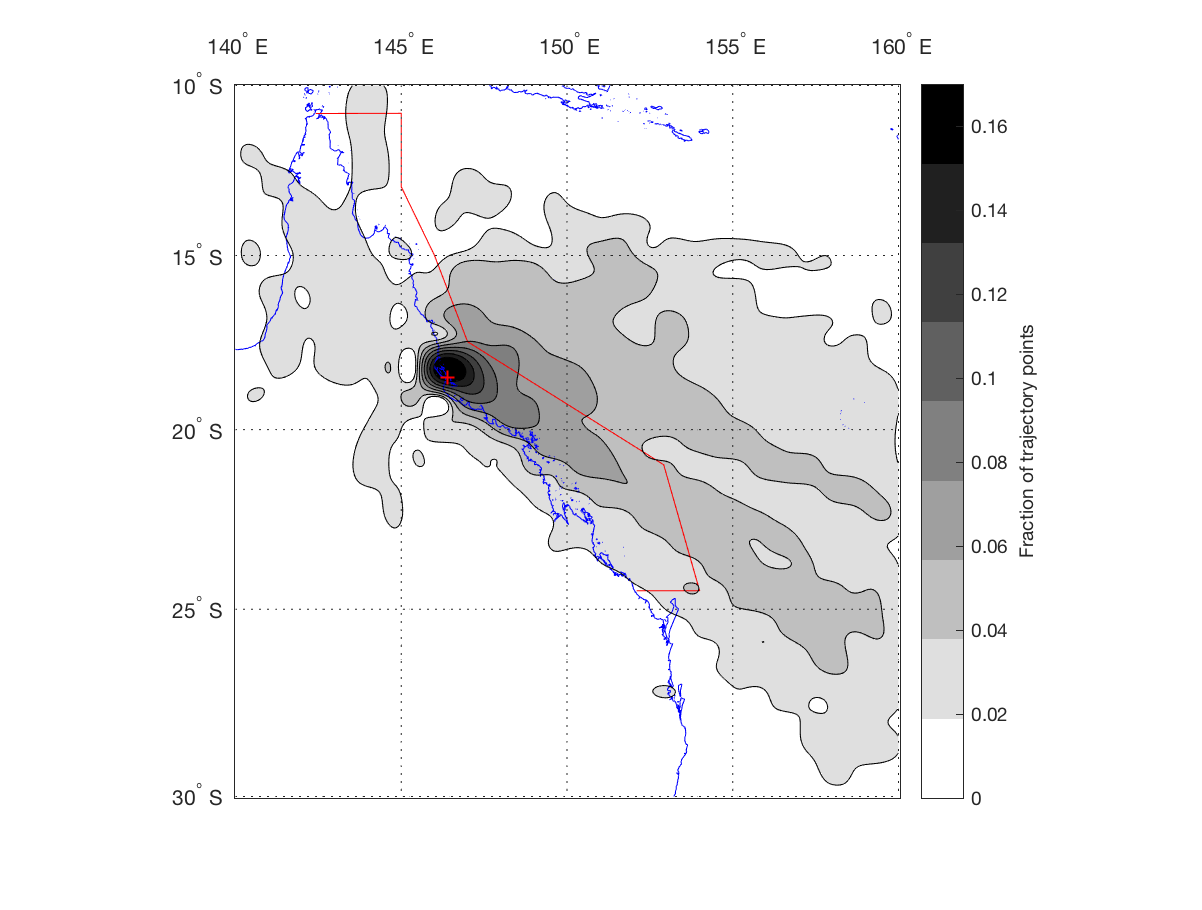
\includegraphics[width=\textwidth]{Fig/Research/BT_Coast/Map_015.eps}
	    \caption{January}
	    \label{subfig:whit}
    \end{subfigure}
    ~
    \begin{subfigure}[b]{0.45\textwidth}
    	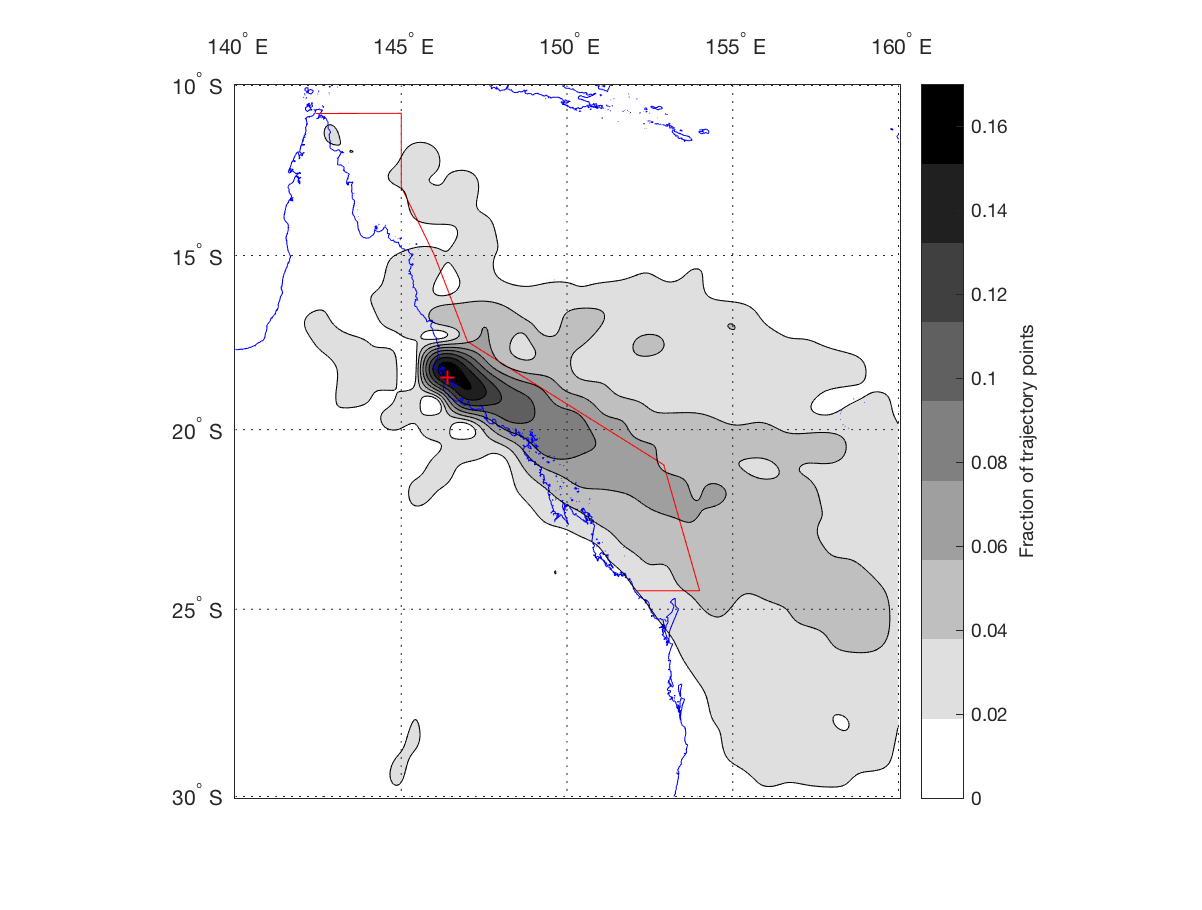
\includegraphics[width=\textwidth]{Fig/Research/BT_Coast/Map_025.eps}
	    \caption{February}
	    \label{subfig:aims}
    \end{subfigure}
    \caption{Continued...}
    \label{fig:btcoastlucjet}
\end{figure}

\begin{figure}[!t]\ContinuedFloat
    \centering
    \begin{subfigure}[b]{0.45\textwidth}
        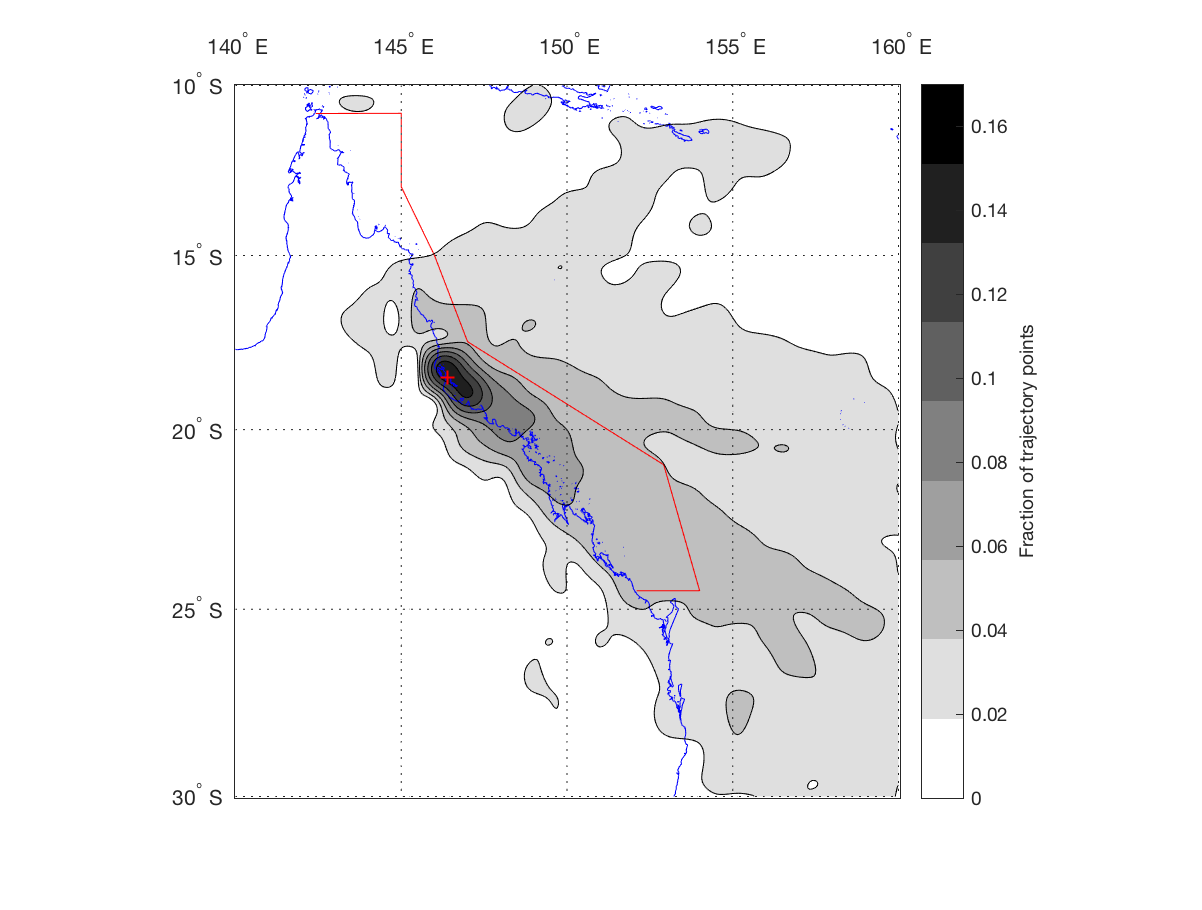
\includegraphics[width=\textwidth]{Fig/Research/BT_Coast/Map_035.eps}
	    \caption{March}
	    \label{subfig:orph}
    \end{subfigure}
	~
	\begin{subfigure}[b]{0.45\textwidth}
		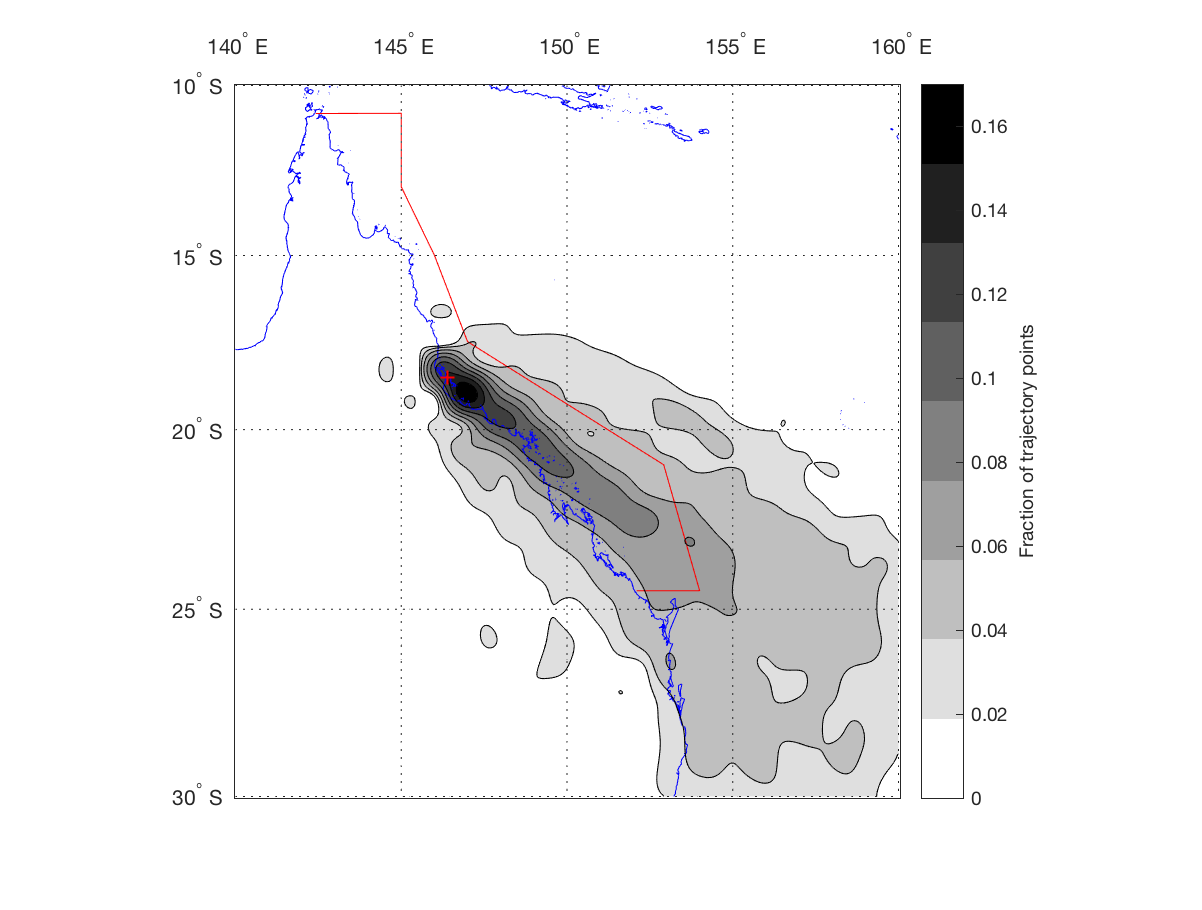
\includegraphics[width=\textwidth]{Fig/Research/BT_Coast/Map_045.eps}
		\caption{April}
		\label{subfig:luci}
	\end{subfigure}
	\\
    \begin{subfigure}[b]{0.45\textwidth}
	    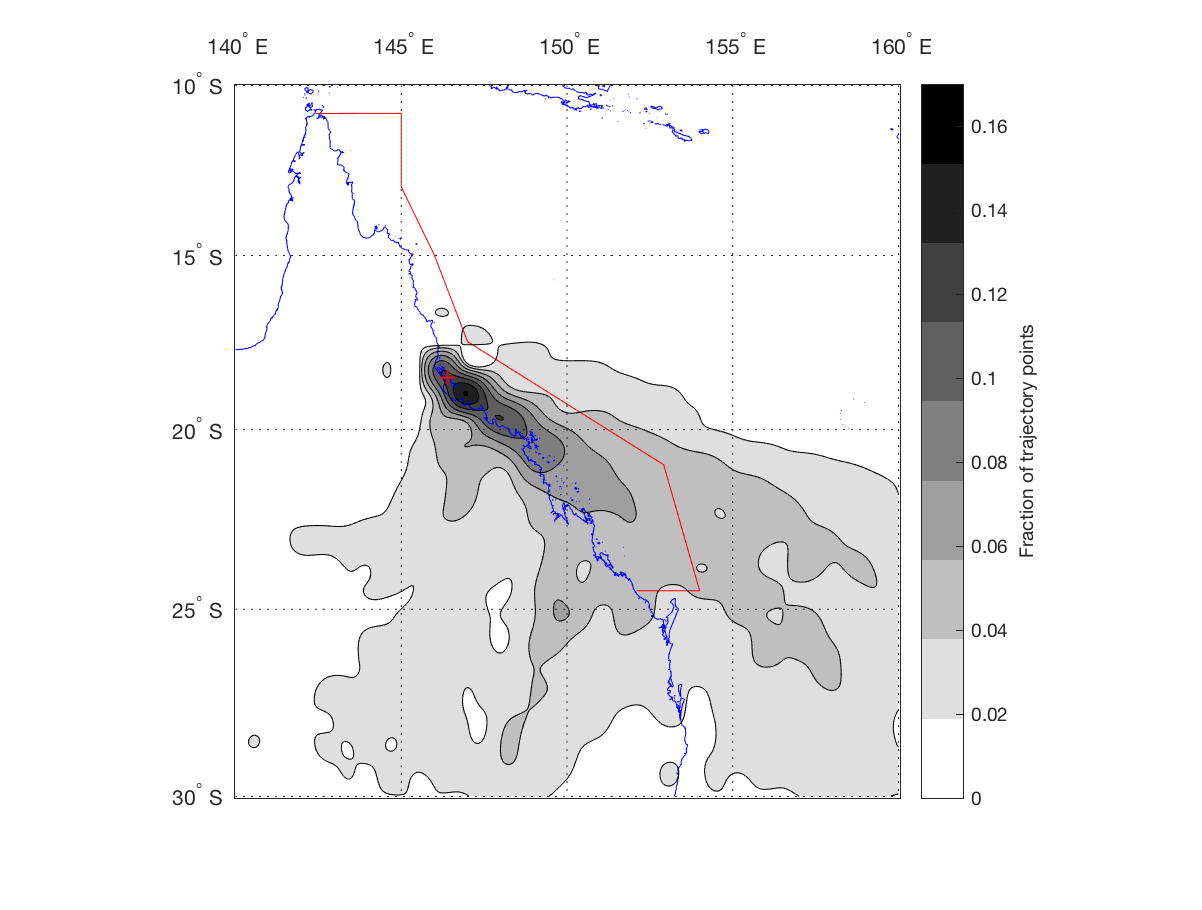
\includegraphics[width=\textwidth]{Fig/Research/BT_Coast/Map_055.eps}
	    \caption{May}
	    \label{subfig:cair}
    \end{subfigure}
    ~
    \begin{subfigure}[b]{0.45\textwidth}
	    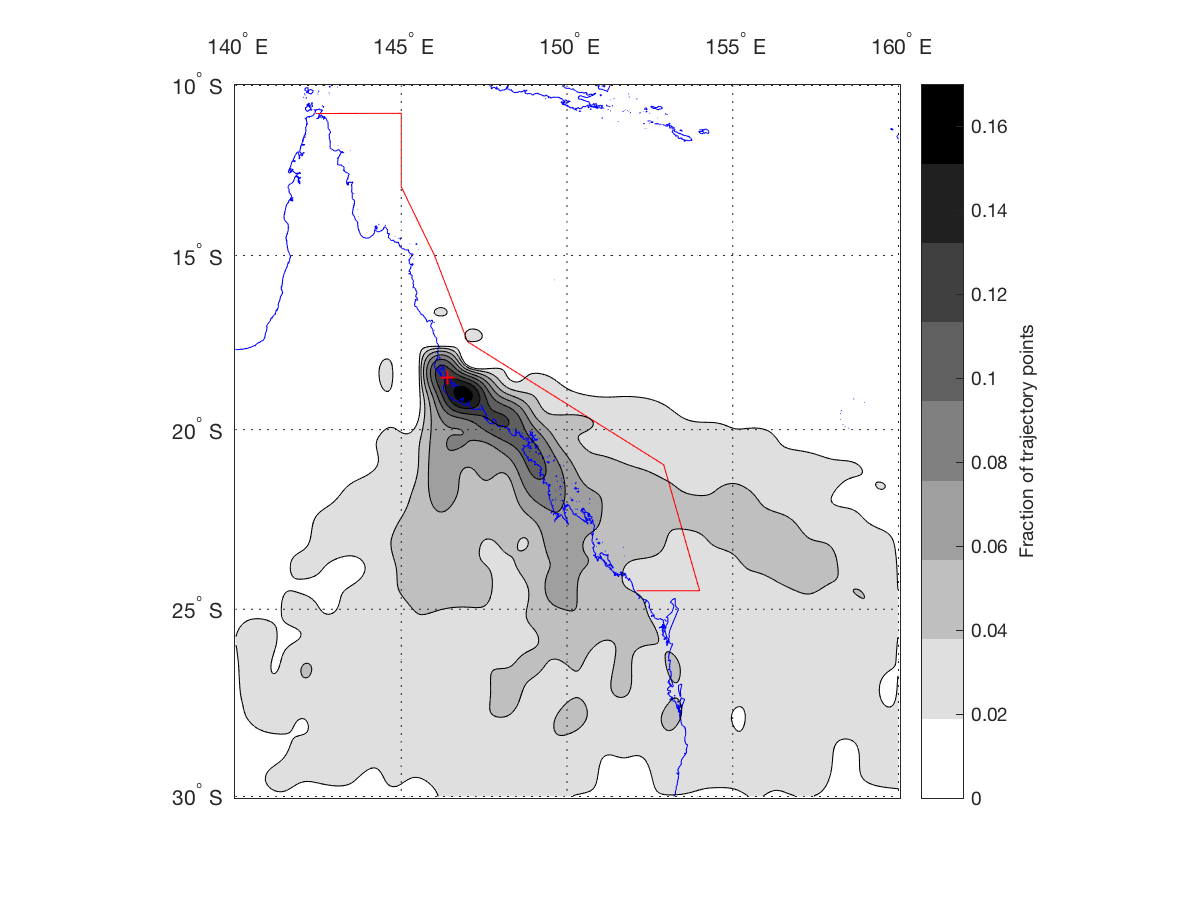
\includegraphics[width=\textwidth]{Fig/Research/BT_Coast/Map_065.eps}
	    \caption{June}
	    \label{subfig:cair}
    \end{subfigure}
	\\
    \begin{subfigure}[b]{0.45\textwidth}
	    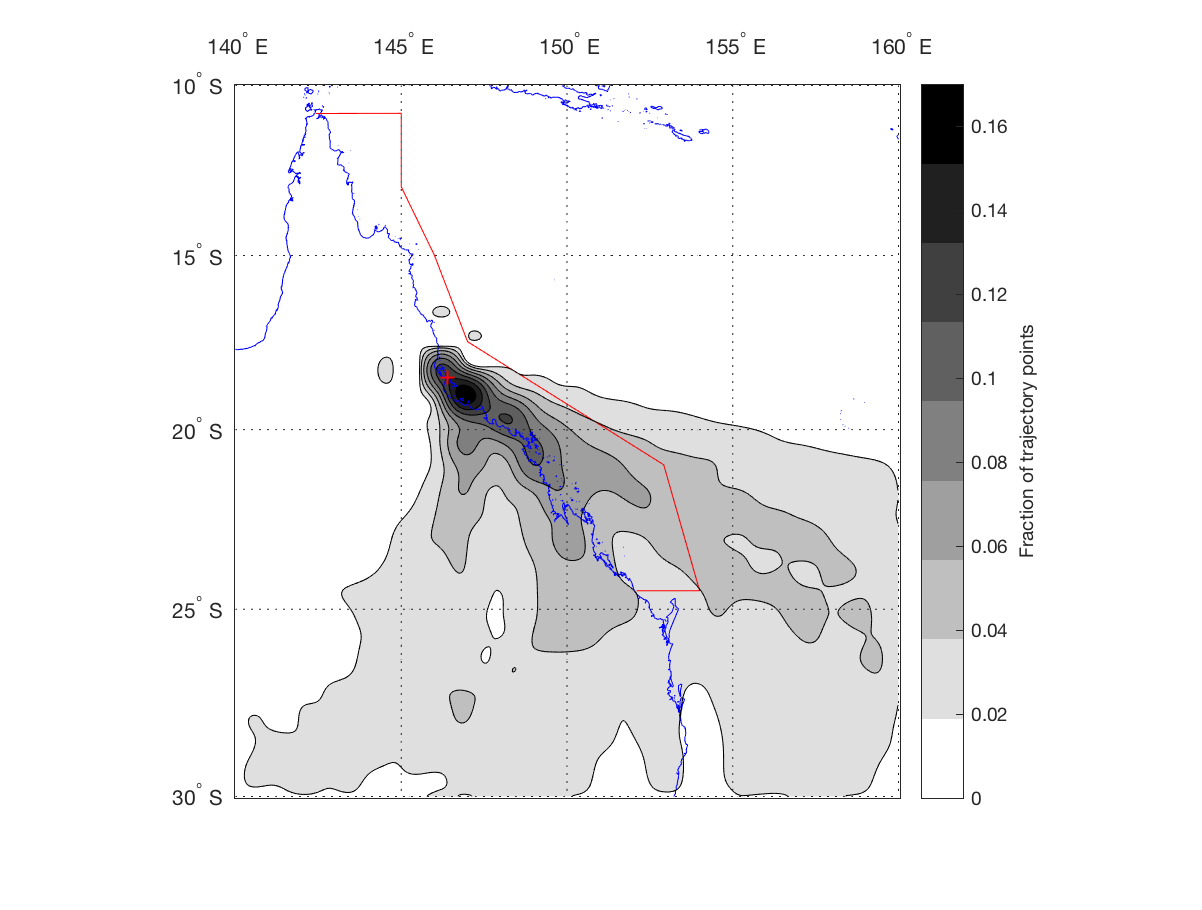
\includegraphics[width=\textwidth]{Fig/Research/BT_Coast/Map_075.eps}
	    \caption{July}
	    \label{subfig:cair}
    \end{subfigure}
    ~
    \begin{subfigure}[b]{0.45\textwidth}
	    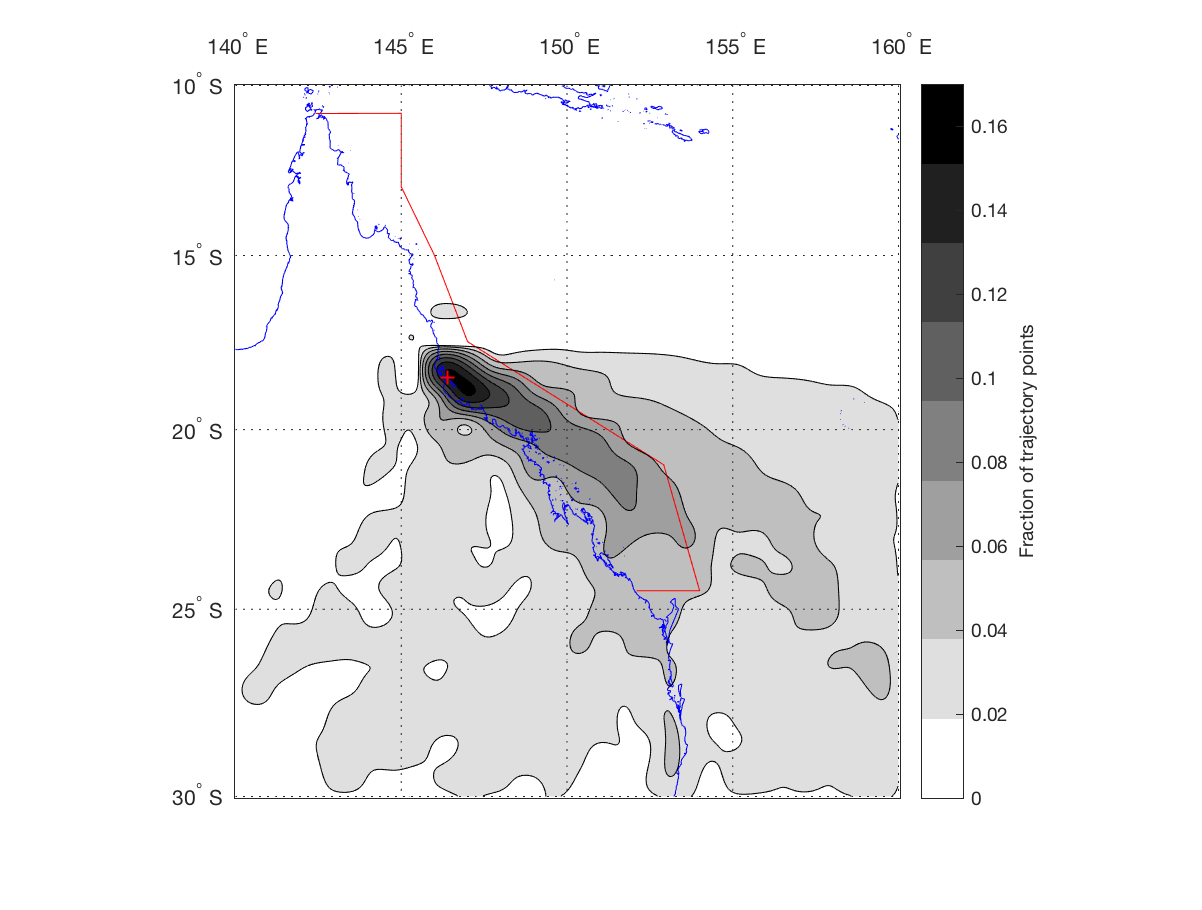
\includegraphics[width=\textwidth]{Fig/Research/BT_Coast/Map_085.eps}
	    \caption{August}
	    \label{subfig:cair}
    \end{subfigure}
    \\
    \begin{subfigure}[b]{0.45\textwidth}
	    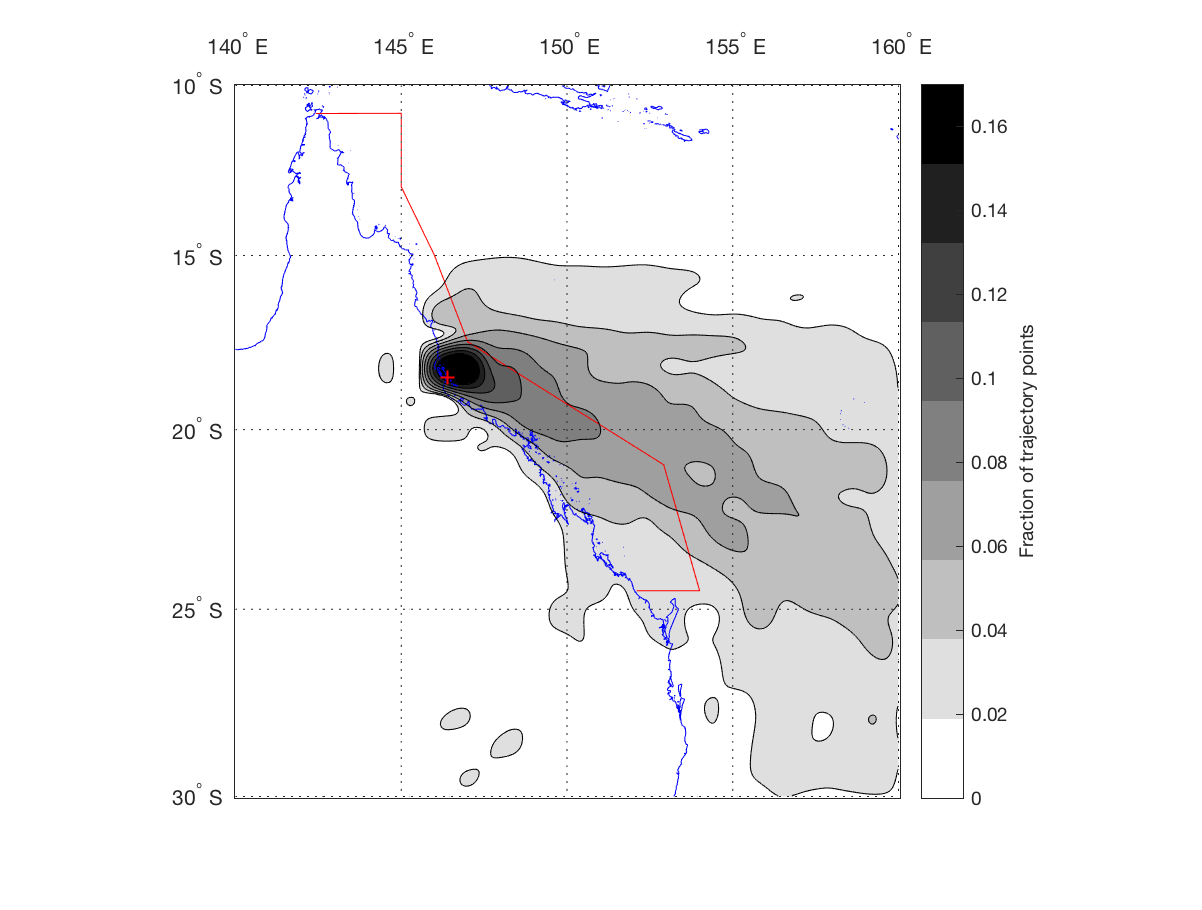
\includegraphics[width=\textwidth]{Fig/Research/BT_Coast/Map_095.eps}
	    \caption{September}
	    \label{subfig:cair}
    \end{subfigure}
    ~
    \begin{subfigure}[b]{0.45\textwidth}
	    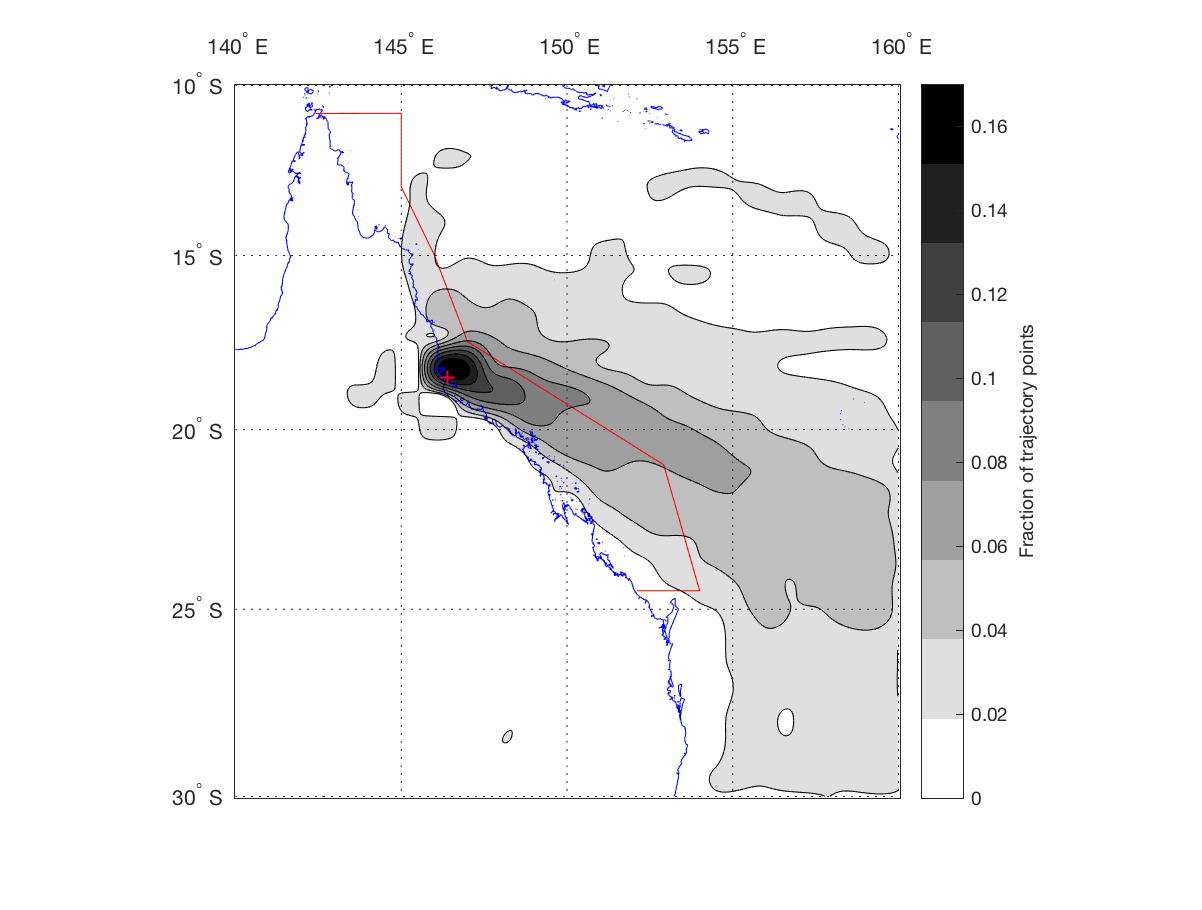
\includegraphics[width=\textwidth]{Fig/Research/BT_Coast/Map_105.eps}
	    \caption{October}
	    \label{subfig:cair}
    \end{subfigure}
    \caption{Continued...}
    \label{fig:btcoastlucjet}
\end{figure}

\clearpage
	
\begin{figure}[!t]\ContinuedFloat
    \centering
    \begin{subfigure}[b]{0.45\textwidth}
	    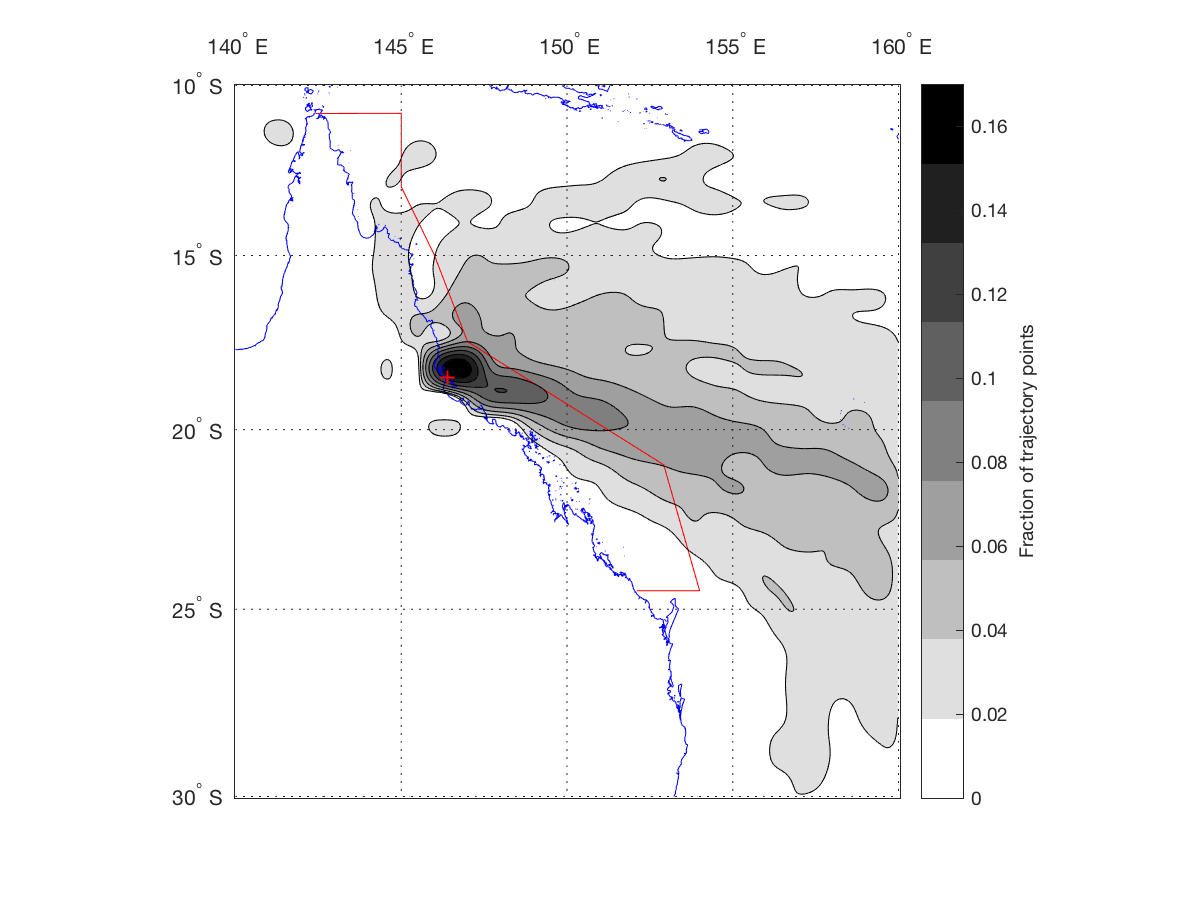
\includegraphics[width=\textwidth]{Fig/Research/BT_Coast/Map_115.eps}
	    \caption{November}
	    \label{subfig:cair}
    \end{subfigure}
    ~
    \begin{subfigure}[b]{0.45\textwidth}
	    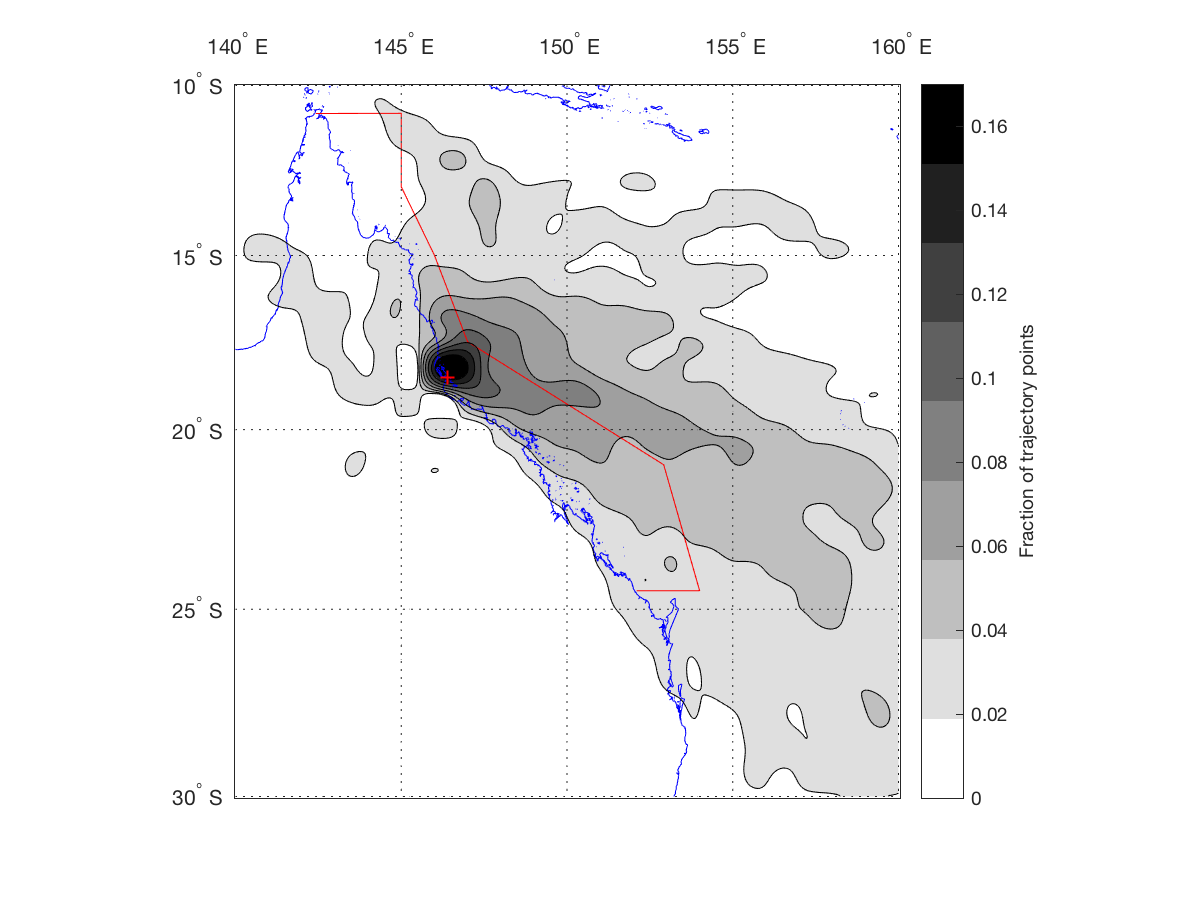
\includegraphics[width=\textwidth]{Fig/Research/BT_Coast/Map_125.eps}
	    \caption{December}
	    \label{subfig:cair}
    \end{subfigure}
    \caption{Interpolated histograms of back trajectory points modelled six times daily, for the months labelled, over the years 2011 to 2014, at Lucinda Jetty -18.520, 146.386.}
    \label{fig:btcoastlucjet}
\end{figure}


%------------------------------------------------------------------------------------------------------------------
% Coast back trajectories for october
\subsection{Coastal Location Back Trajectory Histograms for October}
\label{subsec:coastoctbt}

With guidance from the plots in \cref{fig:btcoastlucjet} and several other groups of year based of plots based on the locations listed in \cref{tab:hysplitlocscoast}, the month of October was selected for further modelling and the experimental campaign. The full ensemble of \gls{hysplit} plots for the coast line locations for October were examined to try and identify sites for setting up equipment (see \cref{fig:btcoastoct}). Again, the best sites have the greatest proportion of back trajectory points over the \gls{gbr}, especially where the reef is dense. A second factor for these coastal locations was anthropogenic sources of aerosols. Sites with less back trajectories coming from inland or along the coastline would likely contain less anthropogenic aerosols. 

\begin{figure}[!hbt]
    \centering
    \begin{subfigure}[b]{0.45\textwidth}
	    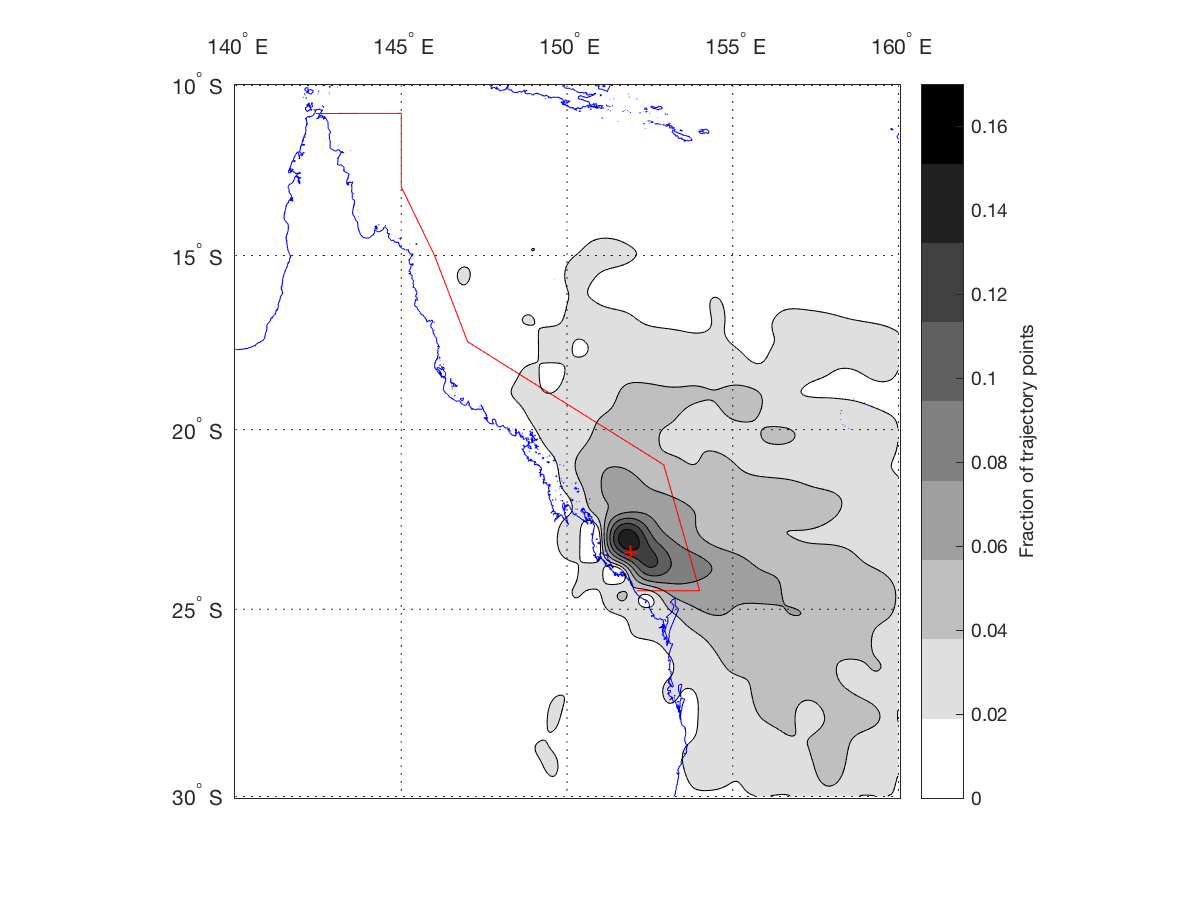
\includegraphics[width=\textwidth]{Fig/Research/BT_Coast/Map_101.eps}
	    \caption{Heron Island -23.442, 151.915}
	    \label{subfig:whit}
    \end{subfigure}
    ~
    \begin{subfigure}[b]{0.45\textwidth}
    	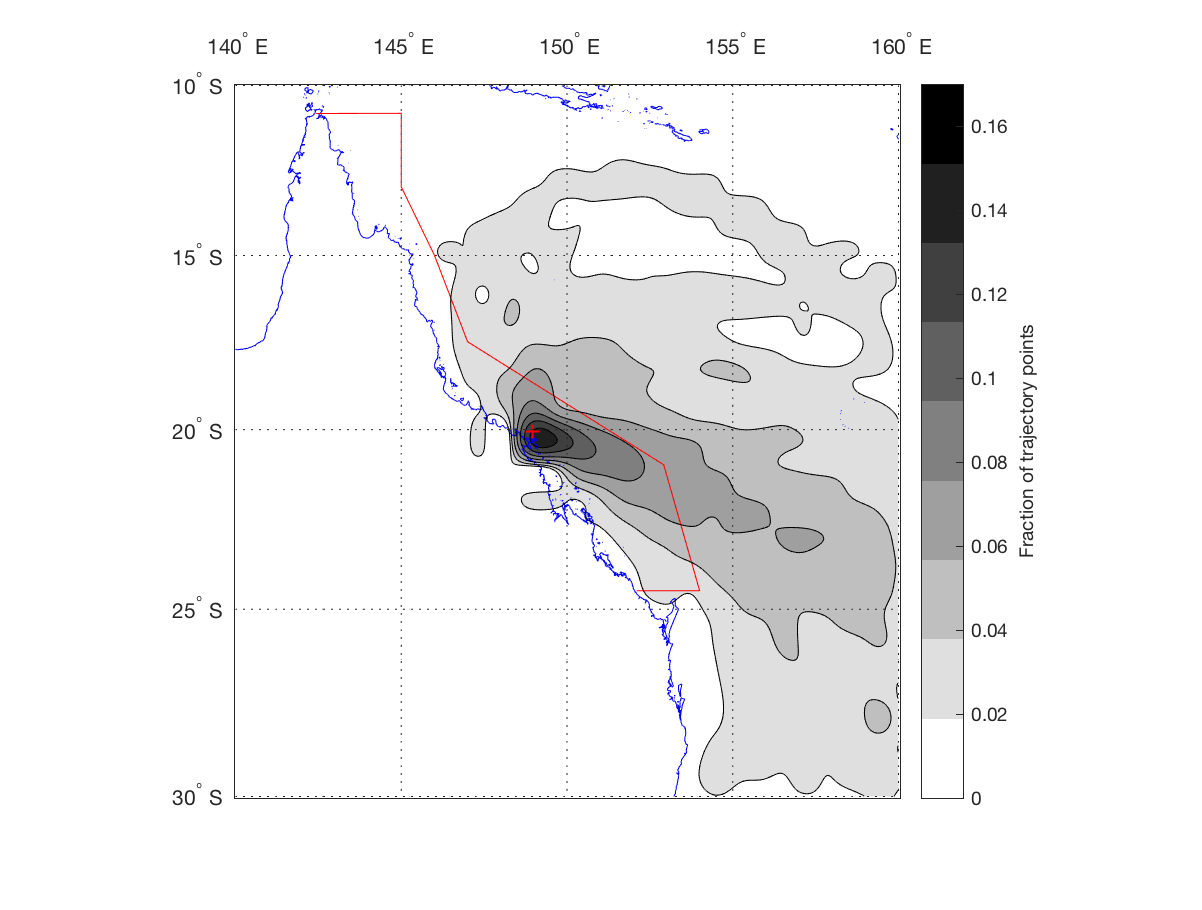
\includegraphics[width=\textwidth]{Fig/Research/BT_Coast/Map_102.eps}
	    \caption{Whitsundays -20.065, 148.949}
	    \label{subfig:aims}
    \end{subfigure}
    \caption{Continued...}
    \label{fig:btcoastlucjet}
\end{figure}

\clearpage
	
\begin{figure}[!t]\ContinuedFloat
    \centering
    \begin{subfigure}[b]{0.45\textwidth}
        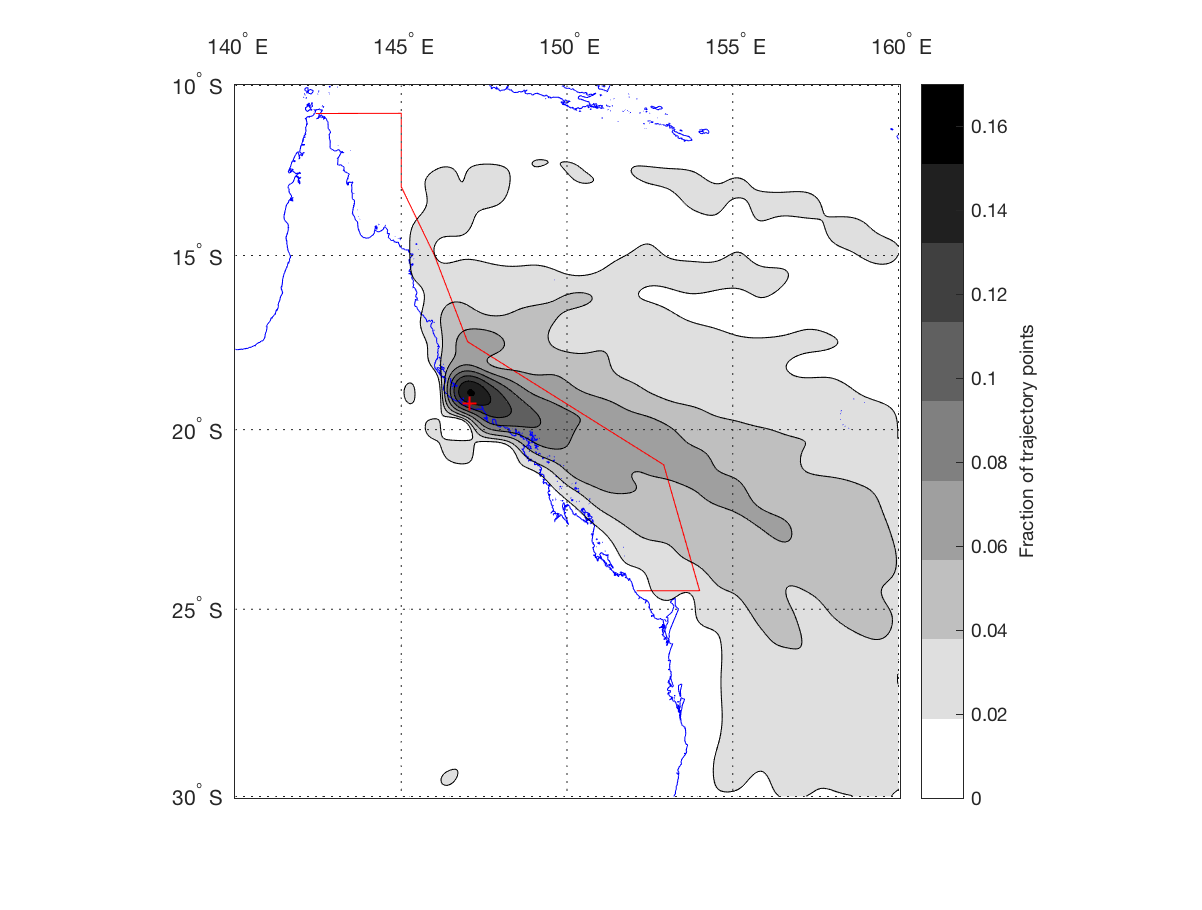
\includegraphics[width=\textwidth]{Fig/Research/BT_Coast/Map_103.eps}
	    \caption{AIMS Cape Ferguson -19.268, 147.057}
	    \label{subfig:orph}
    \end{subfigure}
	~
	\begin{subfigure}[b]{0.45\textwidth}
		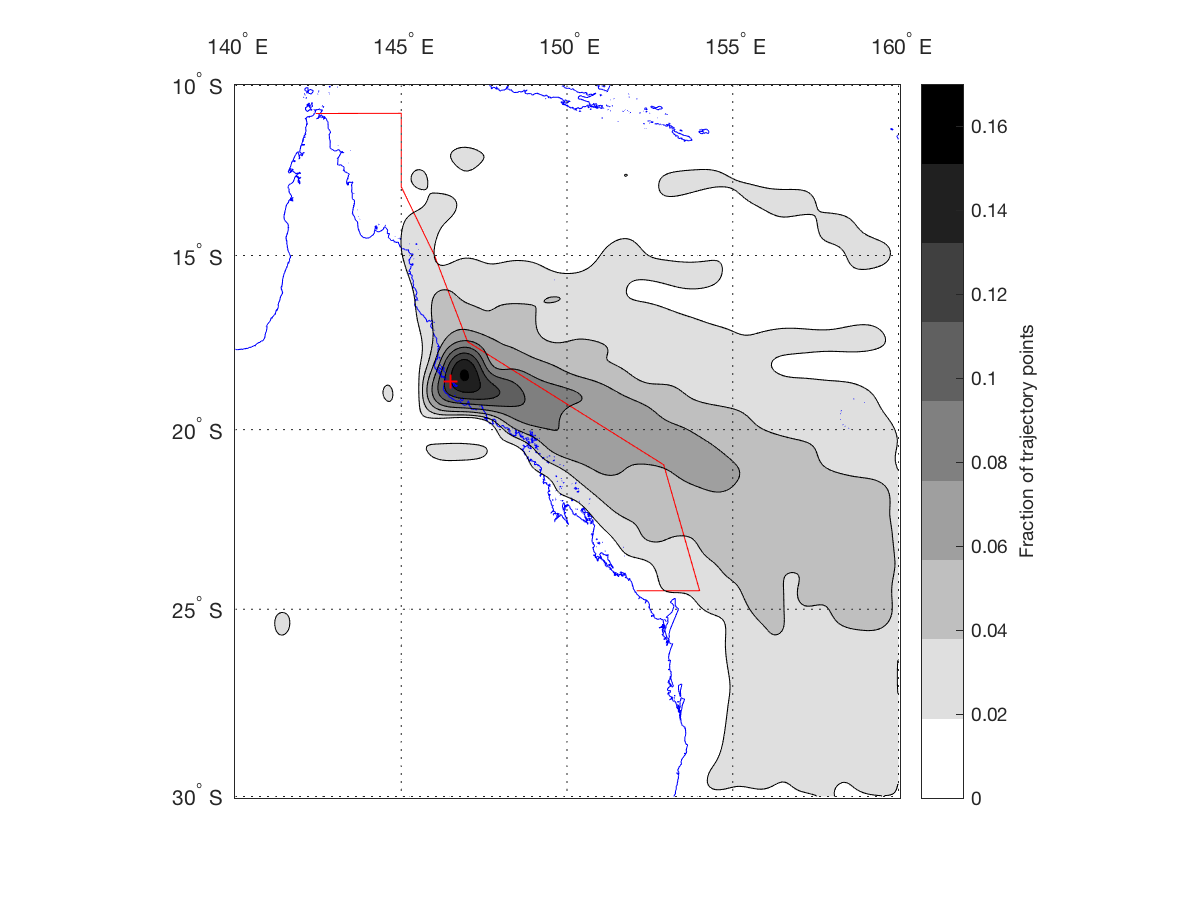
\includegraphics[width=\textwidth]{Fig/Research/BT_Coast/Map_104.eps}
		\caption{Orpheus Island -18.634, 146.500}
		\label{subfig:luci}
	\end{subfigure}
	\\
% 	\caption{Interpolated histograms of back trajectory points modelled six times daily, during October, over the years 2011 to 2014 at the locations labelled.}
%     \label{fig:btcoastoct}
% \end{figure}

% \begin{figure}[!hbt]\ContinuedFloat
%     \centering
    \begin{subfigure}[b]{0.45\textwidth}
	    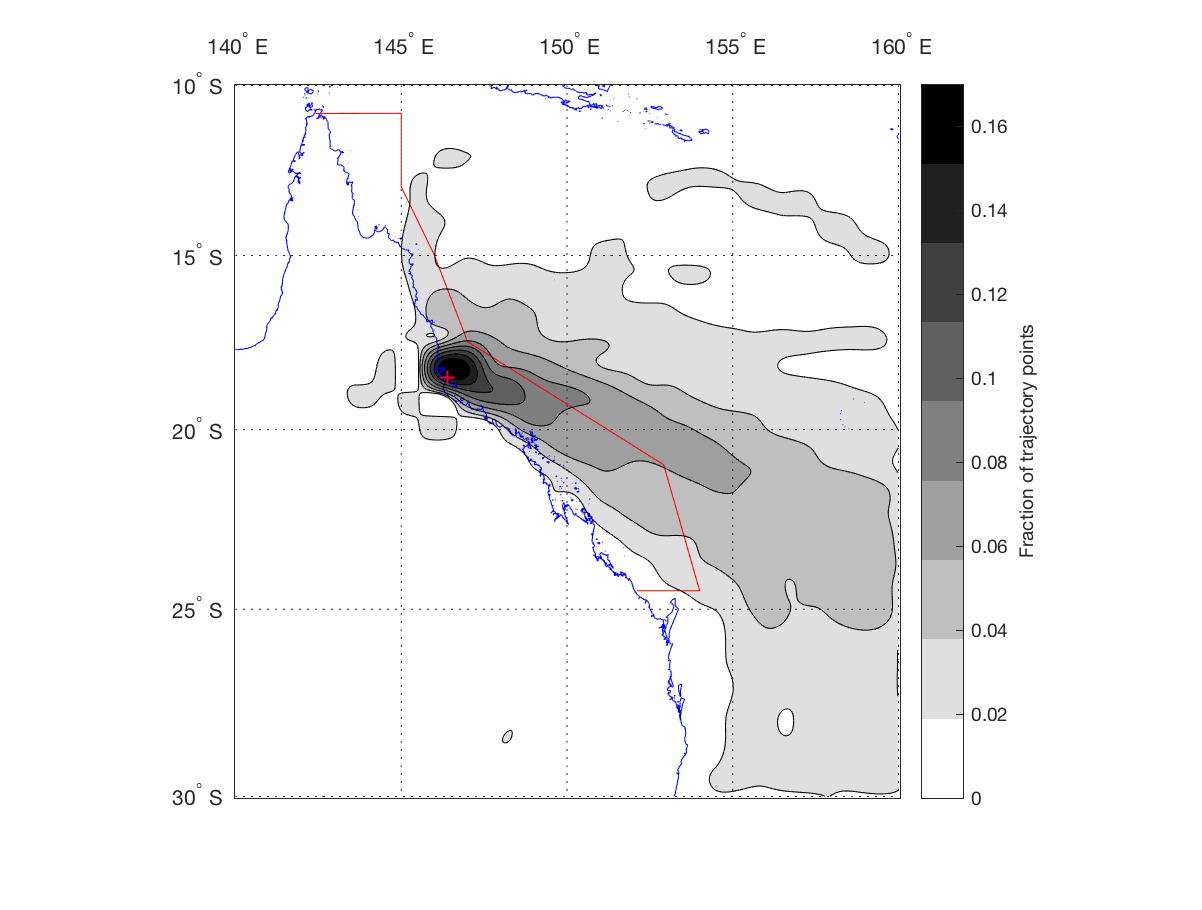
\includegraphics[width=\textwidth]{Fig/Research/BT_Coast/Map_105.eps}
	    \caption{Lucinda Jetty -18.520, 146.386}
	    \label{subfig:cair}
    \end{subfigure}
    ~
    \begin{subfigure}[b]{0.45\textwidth}
	    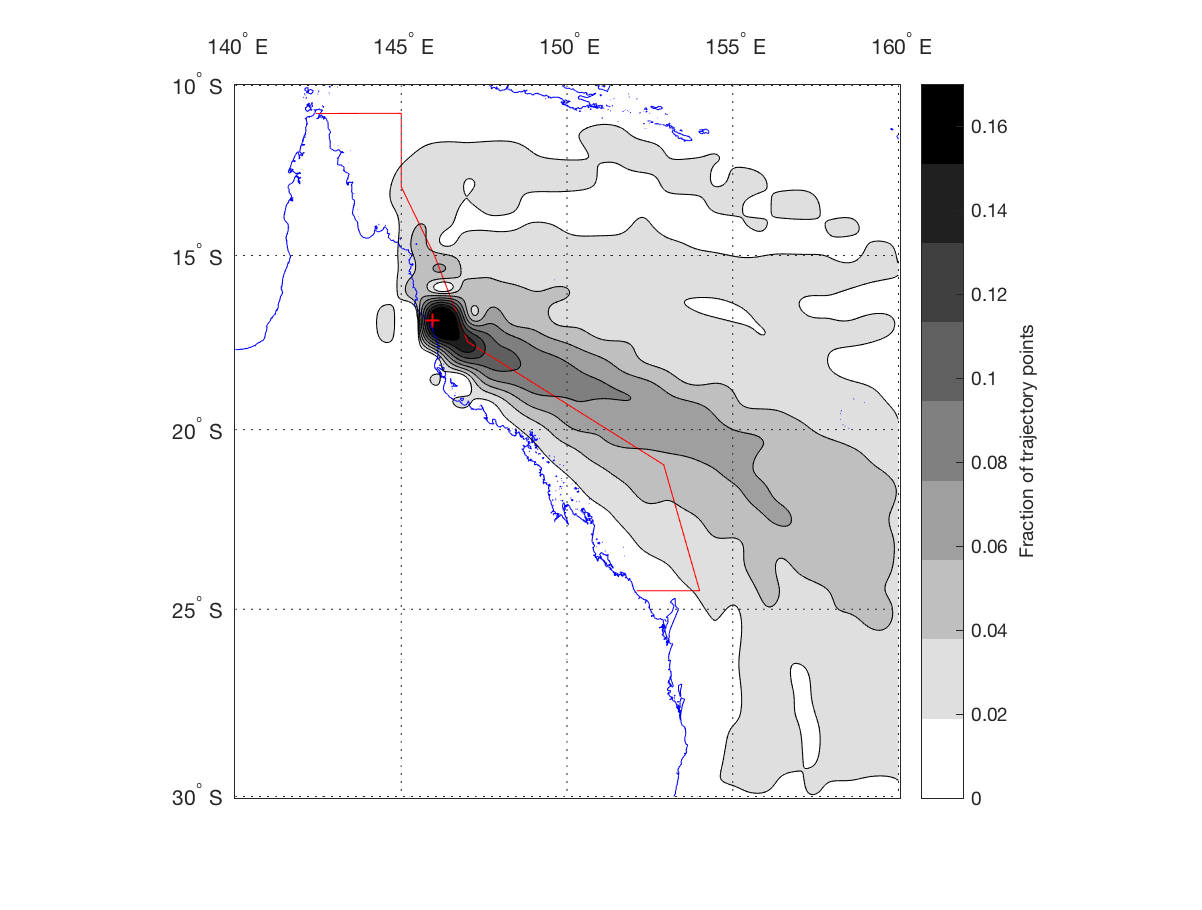
\includegraphics[width=\textwidth]{Fig/Research/BT_Coast/Map_106.eps}
	    \caption{Cairns -16.881, 145.942}
	    \label{subfig:cair}
    \end{subfigure}
	\\
    \begin{subfigure}[b]{0.45\textwidth}
	    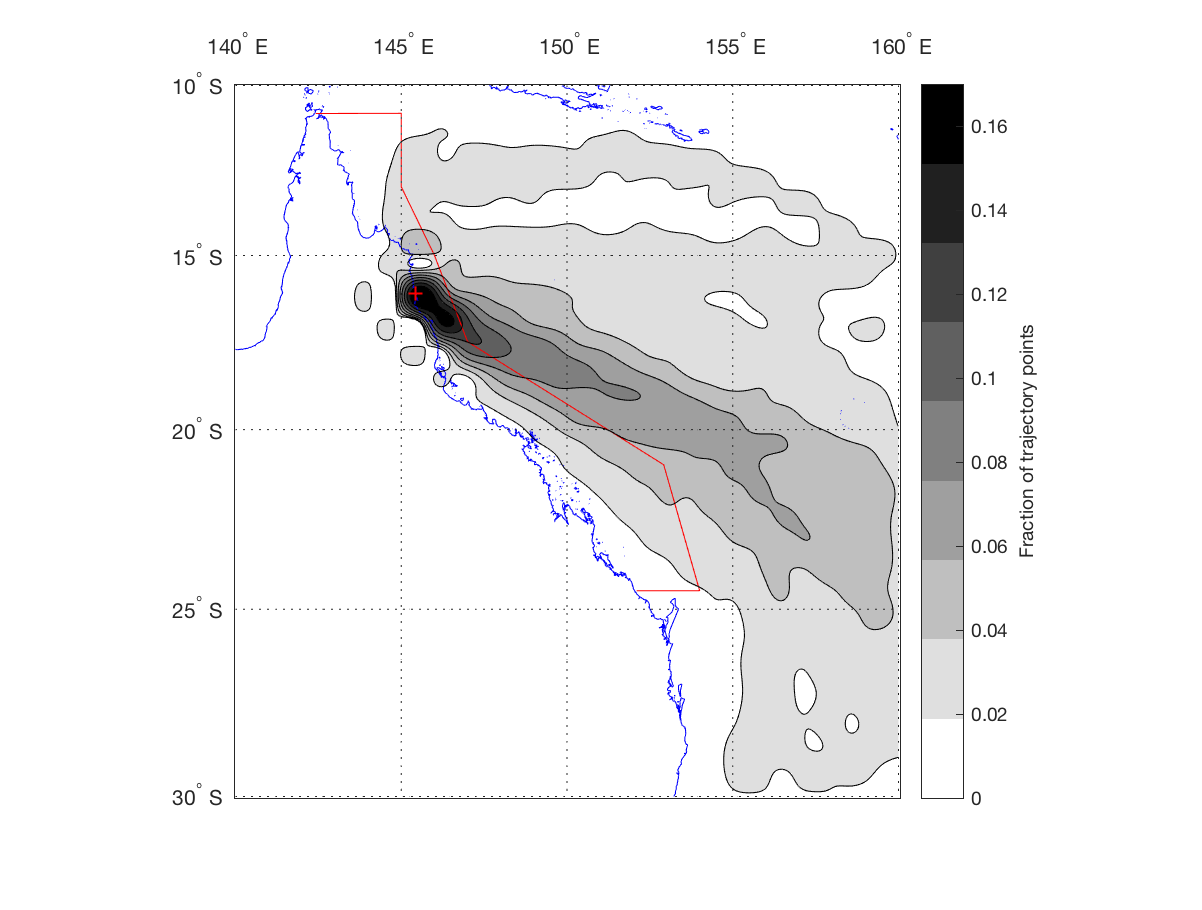
\includegraphics[width=\textwidth]{Fig/Research/BT_Coast/Map_108.eps}
	    \caption{JCU Daintree Obs -16.102, 145.443}
	    \label{subfig:cair}
    \end{subfigure}
    ~
    \begin{subfigure}[b]{0.45\textwidth}
	    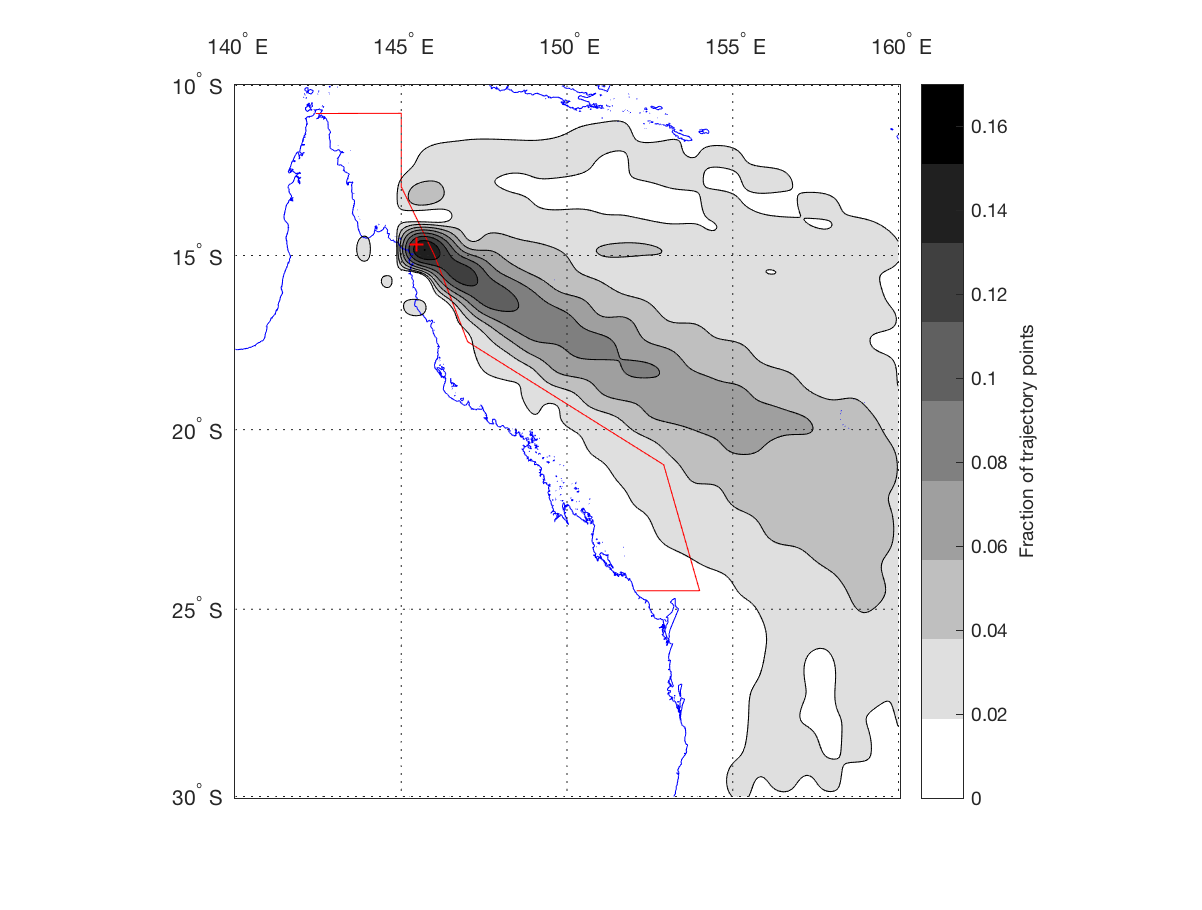
\includegraphics[width=\textwidth]{Fig/Research/BT_Coast/Map_107.eps}
	    \caption{Lizard Island -14.668, 145.448}
	    \label{subfig:cair}
    \end{subfigure}
    \caption{Interpolated histograms of back trajectory points modelled six times daily, during October, over the years 2011 to 2014 at the locations labelled.}
    \label{fig:btcoastoct}
\end{figure}
\clearpage
%------------------------------------------------------------------------------------------------------------------
% Ship back trajectories for october
\subsection{Ship Location Back Trajectory Histograms for October}
\label{subsec:shipoctbt}

For the second part of the experimental campaign the ship would be sampling from in and around the reef. To help guide the selection of the path and stopping locations for the ship, a group of interpolated histogram plots were created using locations off the coast of Queensland (see \cref{tab:hysplitlocsship}). The same criteria for selection used in \cref{subsec:yearbt} was applied.

\begin{figure}[!hbt]
    \centering
    \begin{subfigure}[b]{0.45\textwidth}
	    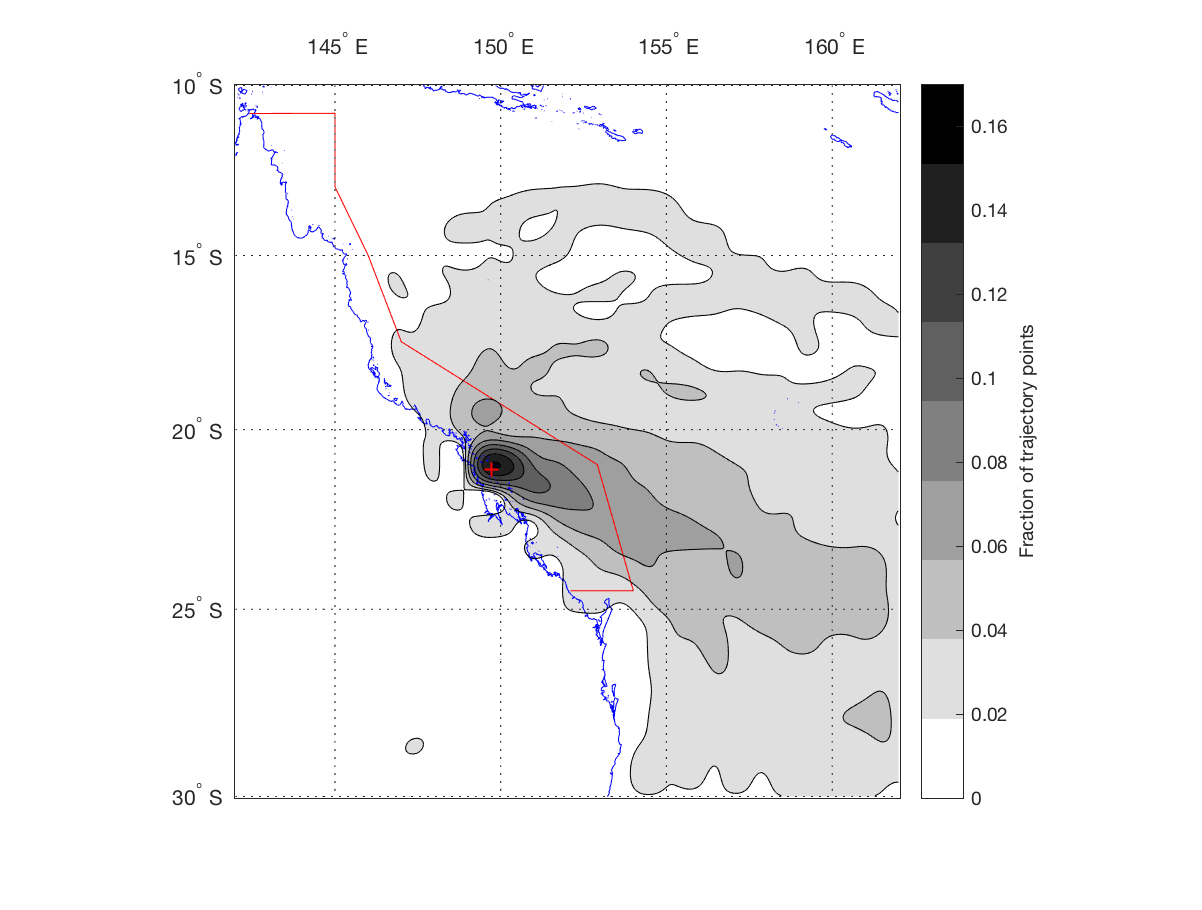
\includegraphics[width=\textwidth]{Fig/Research/BT_Ship/Map_101.eps}
	    \caption{Mackay -21.123, 149.711}
	    \label{subfig:whit}
    \end{subfigure}
    ~
    \begin{subfigure}[b]{0.45\textwidth}
    	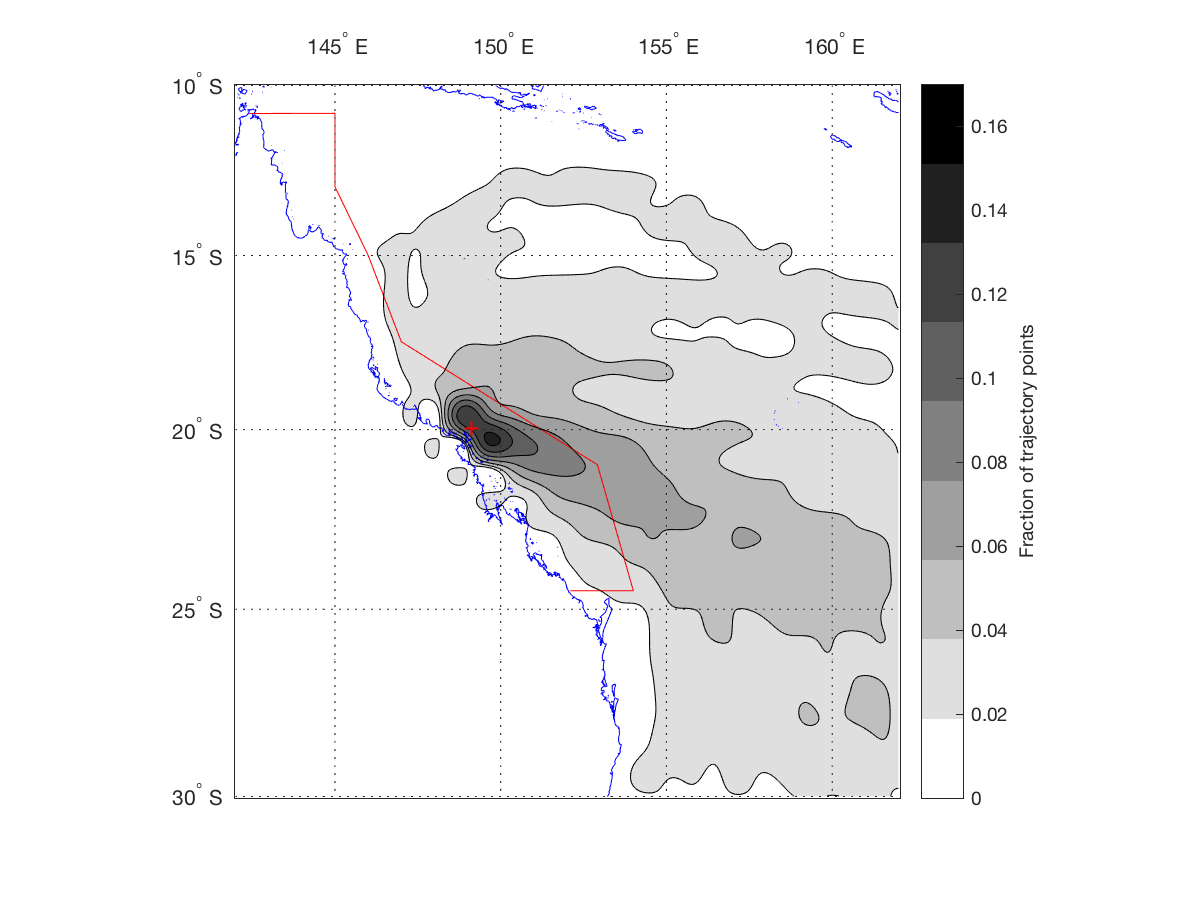
\includegraphics[width=\textwidth]{Fig/Research/BT_Ship/Map_102.eps}
	    \caption{Hamilton -19.982, 149.108}
	    \label{subfig:aims}
    \end{subfigure}
    \\
    \begin{subfigure}[b]{0.45\textwidth}
        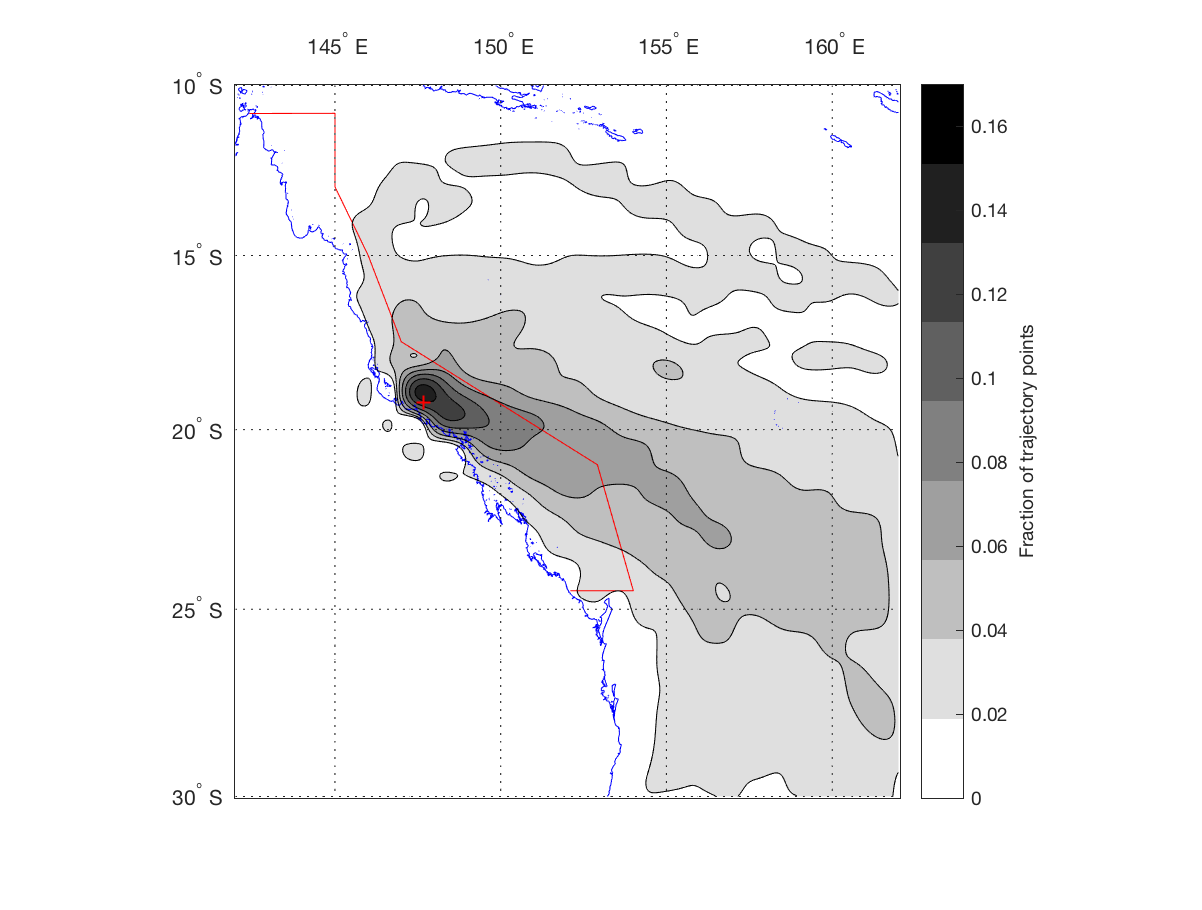
\includegraphics[width=\textwidth]{Fig/Research/BT_Ship/Map_103.eps}
	    \caption{Townsville -19.243, 147.672}
	    \label{subfig:orph}
    \end{subfigure}
	~
	\begin{subfigure}[b]{0.45\textwidth}
		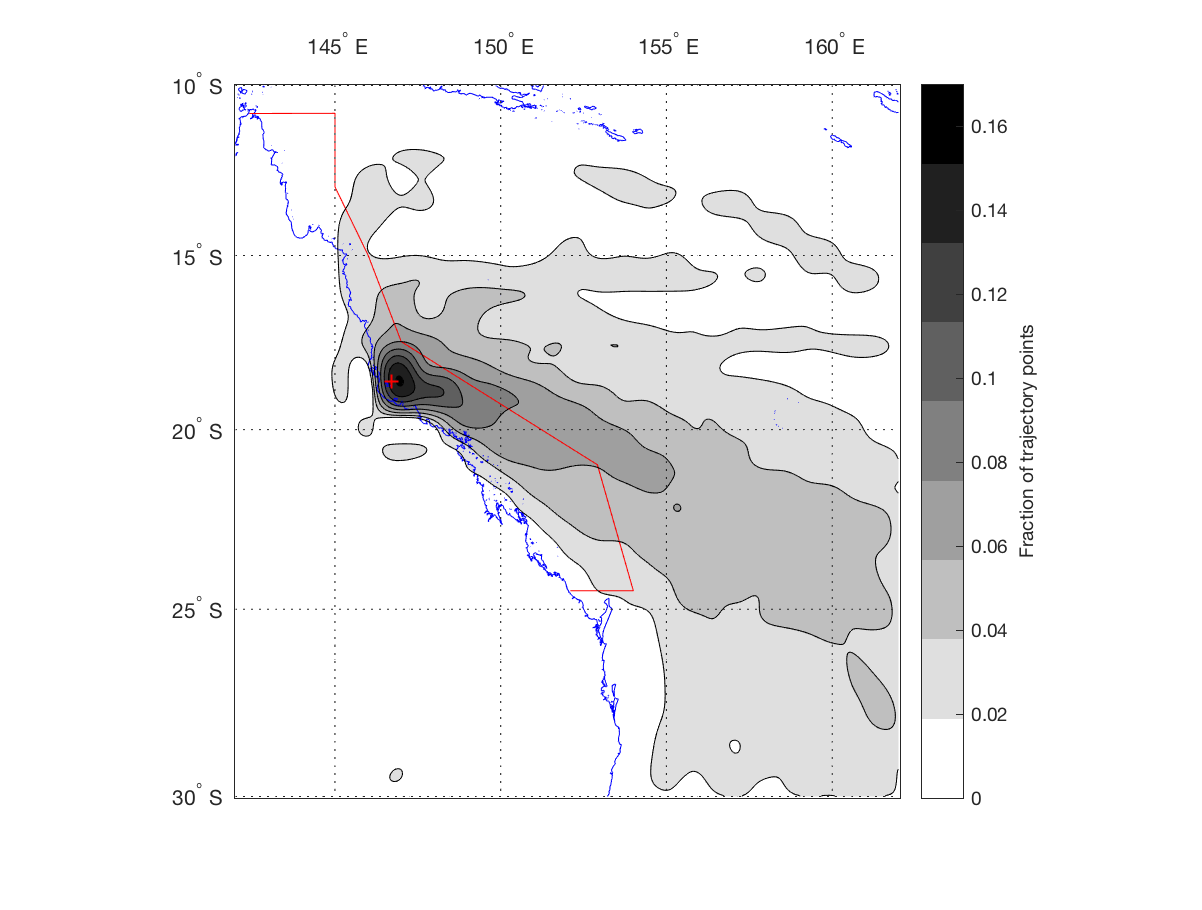
\includegraphics[width=\textwidth]{Fig/Research/BT_Ship/Map_104.eps}
		\caption{Great Palm Isl -18.623, 146.716}
		\label{subfig:luci}
	\end{subfigure}
	\\
    \begin{subfigure}[b]{0.45\textwidth}
	    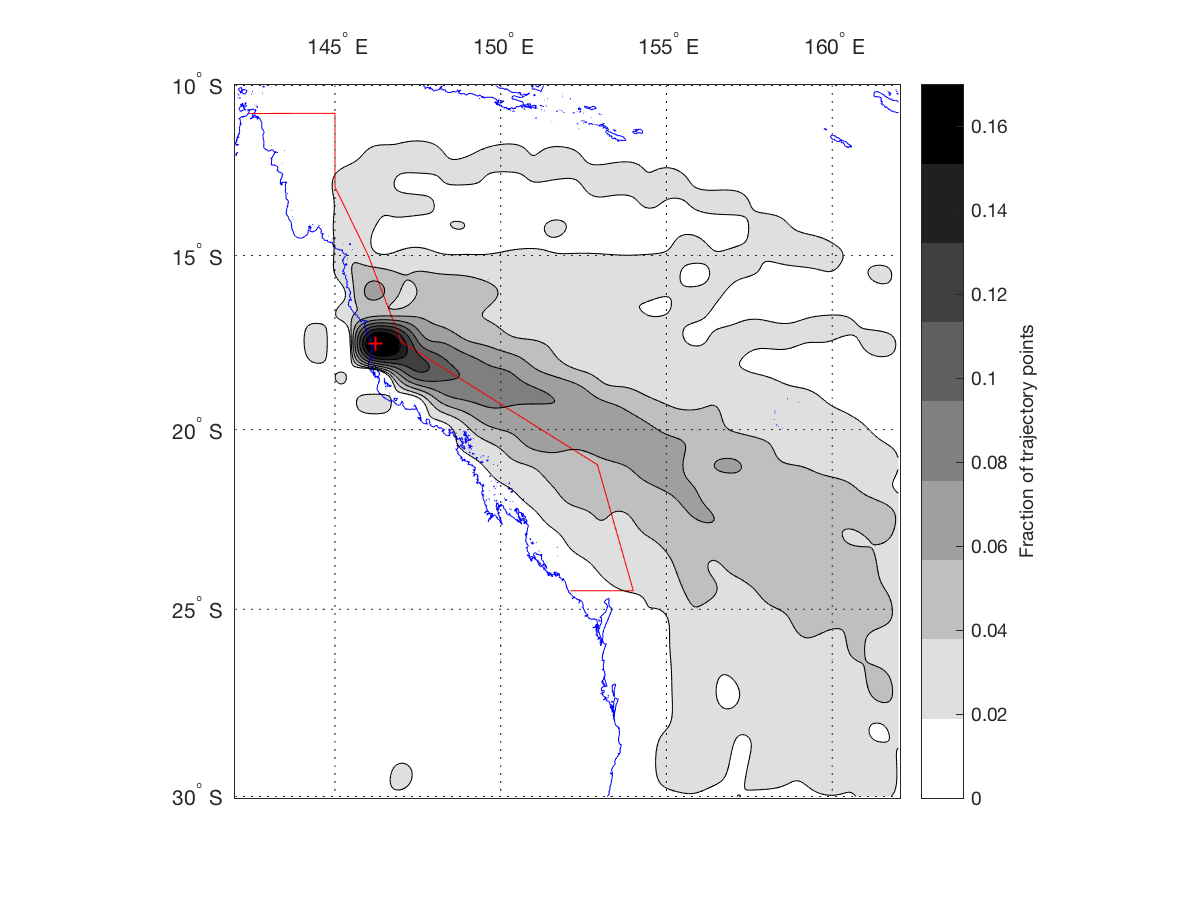
\includegraphics[width=\textwidth]{Fig/Research/BT_Ship/Map_105.eps}
	    \caption{Innisfail -17.533, 146.230}
	    \label{subfig:cair}
    \end{subfigure}
    ~
    \begin{subfigure}[b]{0.45\textwidth}
	    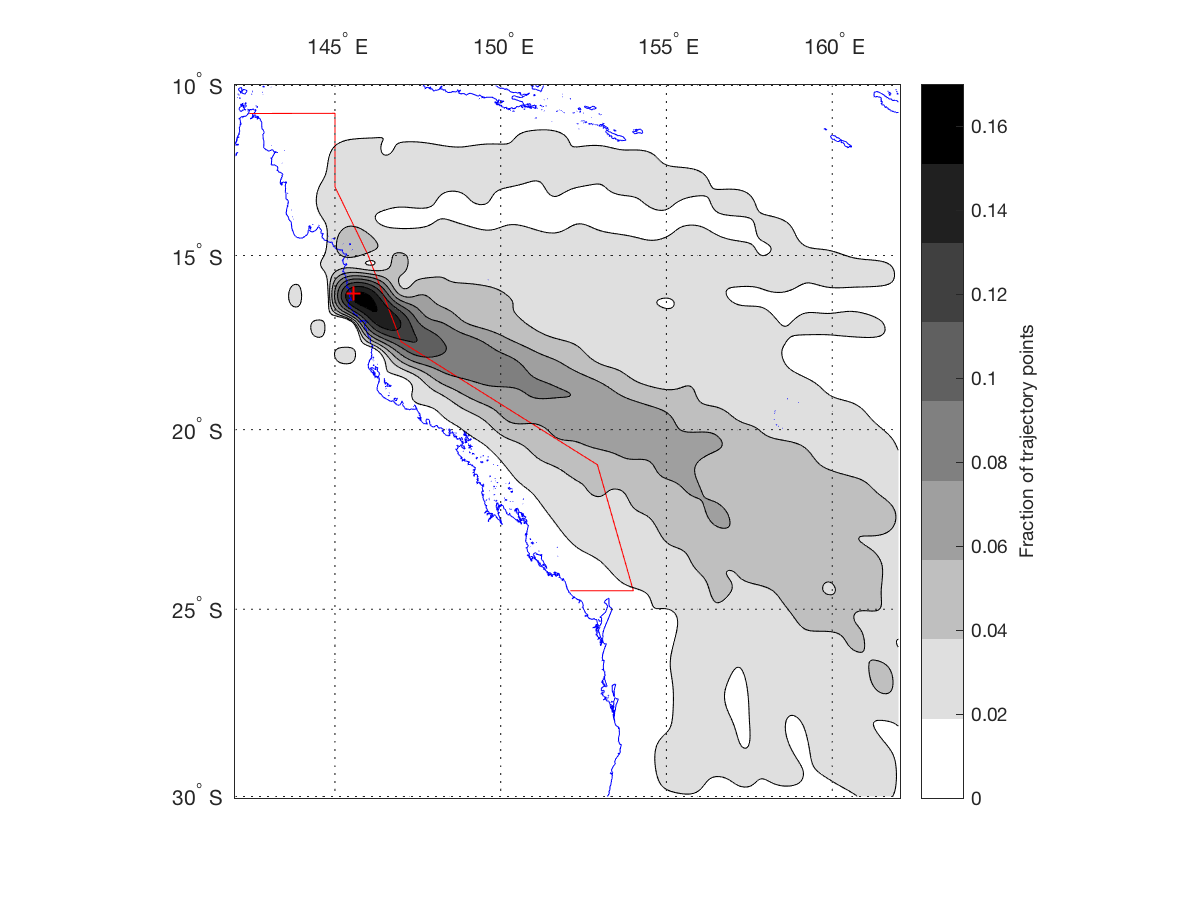
\includegraphics[width=\textwidth]{Fig/Research/BT_Ship/Map_106.eps}
	    \caption{Cape Tribulation -16.093, 145.563}
	    \label{subfig:cair}
    \end{subfigure}
    \caption{Interpolated histograms of back trajectory points modelled six times daily, during October, over the years 2011 to 2014 at the locations labelled.}
    \label{fig:btshipoct}
\end{figure}	

%------------------------------------------------------------------------------------------------------------------
%------------------------------------------------------------------------------------------------------------------
\section{CCAM Validation}
\label{sec:ccamvalid}

The validity of \gls{ccam}'s output is important for understanding the limitations of the model. Interpretation of the output should be modified by these limitations. Measurement data was retrieved from the \gls{bom} and then compared to data from the same locations in the \gls{ccam} output. The variables available were maximum air temperature, minimum air temperature and maximum wind speed. The locations of \gls{bom} stations used in this section can be found in \cref{tab:bomlocs}.

%------------------------------------------------------------------------------------------------------------------
% bom comparison mean residuals
\subsection{Mean Residuals}
\label{subsec:meanresiduals}

To find out if there was a trend to the predictions of \gls{ccam} the mean residuals were calculated. Subtracting the \gls{ccam} data from the available \gls{bom} data and then averaging these residuals for each location produced the values in \cref{tab:bommeanres}. The sign of these values indicates the trend of the model, whether it over (+ve) or under (-ve) predicts the variable in question at that location. They also provide the scale in the units of the measurement.

\begin{table}[tbh!]
	\caption{\textsl{ The mean residuals from a comparison of \gls{ccam} data with \gls{bom} data sampled from a series of Queensland locations. }}
	\centering
		\begin{tabular}{c c c c} \\
			\hline 	\\ 	[-1ex]
			Station				&	Max Temp	&	Min Temp	&	Max Wind 	\\	
			Name 				&	Mean 	&	Mean 	&	Speed Mean 	\\
								&	Residuals ($^{\circ}$C)	&	Residuals ($^{\circ}$C)	&	Residuals (\SI[per-mode=symbol]{}{\meter\per\second})	\\ [1ex]
			\hline	\\	[-1ex]		
			Willis Island		&	-1.61		&	1.35		&	-3.28		\\	
			Low Isles			&	-2.69		&	1.88		&	-3.01		\\	
			Arlington Reef		&	-			&	-			&	-3.15		\\	
			Lihou Reef			&	0.70		&	0.95		&	-2.84		\\	
			Lucinda Point		&	0.01		&	2.06		&	-2.55		\\	
			Hamilton Island		&	-0.53		&	1.65		&	-8.02		\\	
			Mackay				&	-2.51		&	2.19		&	-2.80		\\	
			Middle Percy Island	&	-0.78		&	2.78		&	-5.02		\\	
			Yeppoon				&	-0.87		&	2.15		&	-4.25		\\	
			Heron Island		&	-			&	-			&	-2.27		\\	
			Rundle Island		&	-0.81		&	1.40		&	-2.85		\\	
			Lady Elliot Island	&	-2.69		&	1.57		&	-2.40		\\	[1ex]
			\hline \\
		\end{tabular}
	\label{tab:bommeanres}
\end{table}

%------------------------------------------------------------------------------------------------------------------
% bom comparison plots
\subsection{Comparison of BOM and CCAM Data}
\label{subsec:compplots}

The percentage difference between the \gls{ccam} and \gls{bom} values were calculated for the available variables and station locations. Taking the mean of these percentage differences over time for each location provides an indicator for how well \gls{ccam} is simulating the interactions surrounding these atmospheric properties. These \gls{mpd} values measure the normalised distance allowing comparison with each other.

\begin{table}[tbh!]
	\caption{\textsl{ The Mean Percentage Differences, calculated from a comparison of \gls{ccam} data with \gls{bom} data, sampled from a series of Queensland locations. }}
	\centering
		\begin{tabular}{c c c c} \\
			\hline 	\\ 	[-1ex]
			Station	&	Max Temp			&	Min Temp			&	Max Wind Speed		\\	
			Name	&	Mean Percentage		&	Mean Percentage		&	Mean Percentage		\\	
					&	Difference			&	Difference			&	Difference			\\	[1ex]
			\hline	\\	[-1ex]												
			Willis Island		&	5.74 $\pm$ 2.41		&	6.64 $\pm$ 4.86		&	23.3 $\pm$ 9.8		\\	
			Low Isles			&	9.16 $\pm$ 3.15		&	8.44 $\pm$ 4.34		&	22.8 $\pm$ 10.0		\\	
			Arlington Reef		&	-					&	-	 	 			&	22.7 $\pm$ 11.4		\\	
			Lihou Reef			&	3.08 $\pm$ 1.35		&	5.54 $\pm$ 3.76		&	21.5 $\pm$ 11.0		\\	
			Lucinda Point		&	2.77 $\pm$ 1.95		&	9.74 $\pm$ 5.87		&	20.8 $\pm$ 11.0		\\	
			Hamilton Island		&	2.83 $\pm$ 1.92		&	7.91 $\pm$ 4.56		&	55.9 $\pm$ 6.5		\\	
			Mackay				&	8.92 $\pm$ 2.56		&	13.0 $\pm$ 9.89		&	26.7 $\pm$ 11.2		\\	
			Middle Percy Island	&	3.26 $\pm$ 1.90		&	14.0 $\pm$ 4.20		&	38.6 $\pm$ 11.4		\\	
			Yeppoon				&	3.87 $\pm$ 1.91		&	12.0 $\pm$ 10.2		&	36.8 $\pm$ 7.7		\\	
			Heron Island		&	-					&	-		 			&	21.7 $\pm$ 9.1		\\	
			Rundle Island		&	3.81 $\pm$ 3.88		&	6.76 $\pm$ 3.19		&	22.7 $\pm$ 10.0		\\	
			Lady Elliot Island	&	10.2 $\pm$ 2.6		&	7.93 $\pm$ 5.30		&	21.1 $\pm$ 10.0		\\	[1ex]
			\hline \\
		\end{tabular}
	\label{tab:bompercdiff}
\end{table}

The most direct way of comparing the \gls{bom} and \gls{ccam} data is to plot them against each other, over time. A comparison of the shapes of the graphs can be made along with their distance from each other. Spikes and noise are also obvious. The locations with the highest and lowest \gls{mpd}s, for each measurement, were chosen as a sample from \cref{tab:bompercdiff}. They show where the values in \cref{tab:bompercdiff} and \cref{subsec:meanresiduals} came from and how much variation there is between locations. 

\begin{figure}[!hbt]
    \centering
    \begin{subfigure}[b]{0.45\textwidth}
    	\includegraphics[width=\textwidth]{Fig/Research/BomComparison/MaxTemp_vs_Time_Lucinda_Point.eps}
	    \caption{Max Temp, Lowest \gls{mpd}}
	    \label{subfig:maxtlucpoint}
    \end{subfigure}
    ~~~
    \begin{subfigure}[b]{0.45\textwidth}
    	\includegraphics[width=\textwidth]{Fig/Research/BomComparison/MaxTemp_vs_Time_Lady_Elliot_Island.eps}
	    \caption{Max Temp, Highest \gls{mpd}}
	    \label{subfig:maxtladyelliot}
    \end{subfigure}
    \\
    \vspace{0.5cm}
    \begin{subfigure}[b]{0.45\textwidth}
        \includegraphics[width=\textwidth]{Fig/Research/BomComparison/MinTemp_vs_Time_Lihou_Reef.eps}
	    \caption{Min Temp, Lowest \gls{mpd}}
	    \label{subfig:maxtlihoureef}
    \end{subfigure}
	~~~
	\begin{subfigure}[b]{0.45\textwidth}
		\includegraphics[width=\textwidth]{Fig/Research/BomComparison/MinTemp_vs_Time_Middle_Percy_Island.eps}
		\caption{Min Temp, Highest \gls{mpd}}
		\label{subfig:maxtmiddlepercy}
	\end{subfigure}
	\\
	\vspace{0.5cm}
    \begin{subfigure}[b]{0.45\textwidth}
        \includegraphics[width=\textwidth]{Fig/Research/BomComparison/MaxWind_vs_Time_Lucinda_Point.eps}
	    \caption{Max Wind Speed, Lowest \gls{mpd}}
	    \label{subfig:maxtluci}
    \end{subfigure}
	~~~
	\begin{subfigure}[b]{0.45\textwidth}
		\includegraphics[width=\textwidth]{Fig/Research/BomComparison/MaxWind_vs_Time_Hamilton_Island.eps}
		\caption{Max Wind Speed, Highest \gls{mpd}}
		\label{subfig:maxthamilton}
	\end{subfigure}
    \caption{A comparison of \gls{bom} station data and data produced by \gls{ccam}. Locations were selected based on the lowest (left) and highest (right) mean of percentage differences between the two data sets (taken from \cref{tab:bompercdiff}). The variables are the Maximum and Minimum daily Air Temperatures near the surface, and the Maximum daily \SI{10}{\m} Wind Speed.}
    \label{fig:bomcompdata}
\end{figure}

\clearpage
%------------------------------------------------------------------------------------------------------------------
%------------------------------------------------------------------------------------------------------------------
\section{CCAM Output}
\label{sec:ccamoutput}

As discussed in \cref{subsec:datared} the output from \gls{ccam} must be reduced to be able to plot it. The region of interest was chosen as the \gls{gbr} for collapsing the spatial dimensions. The points within it were extracted and averaged for each hour in the model. To produce the maps, the hourly values of the time dimension, for each point in the map, were averaged and these points were gridded onto the final \gls{ccam} domain.

Each of the variables examined in this section explore the output of \gls{ccam}. There is a particular focus on parameters of the atmosphere that influence \gls{dms} production, its movement and transformation, and its potential for effecting cloud coverage and rain.

%------------------------------------------------------------------------------------------------------------------
\subsection{Surface and Pressure Level Heights}
\label{subsec:heights}

As \gls{ccam} uses pressure Levels rather than height for its vertical axis, seeing the relationship between the pressure Levels and the geopotential height is important for drawing conclusions requiring the actual height. This relationship can be seen in \cref{fig:geoheightvpress}. The height of the surface is also important as it shows the location of surface artefacts like mountain ranges (see \cref{fig:zsmap}).
%\clearpage
\begin{figure}[!hbt]
    \centering
    \includegraphics[width=0.7\textwidth]{Fig/Research/CCAM/GBRnTimeAveragedPlot_GeoHeight.eps}
    \caption{ The Geopotential Height averaged from all points within the \gls{gbr} and also averaged over time then plotted against the modelled Pressure Levels. }
    \label{fig:geoheightvpress}
\end{figure}

\begin{figure}[!hbt]
    \centering
    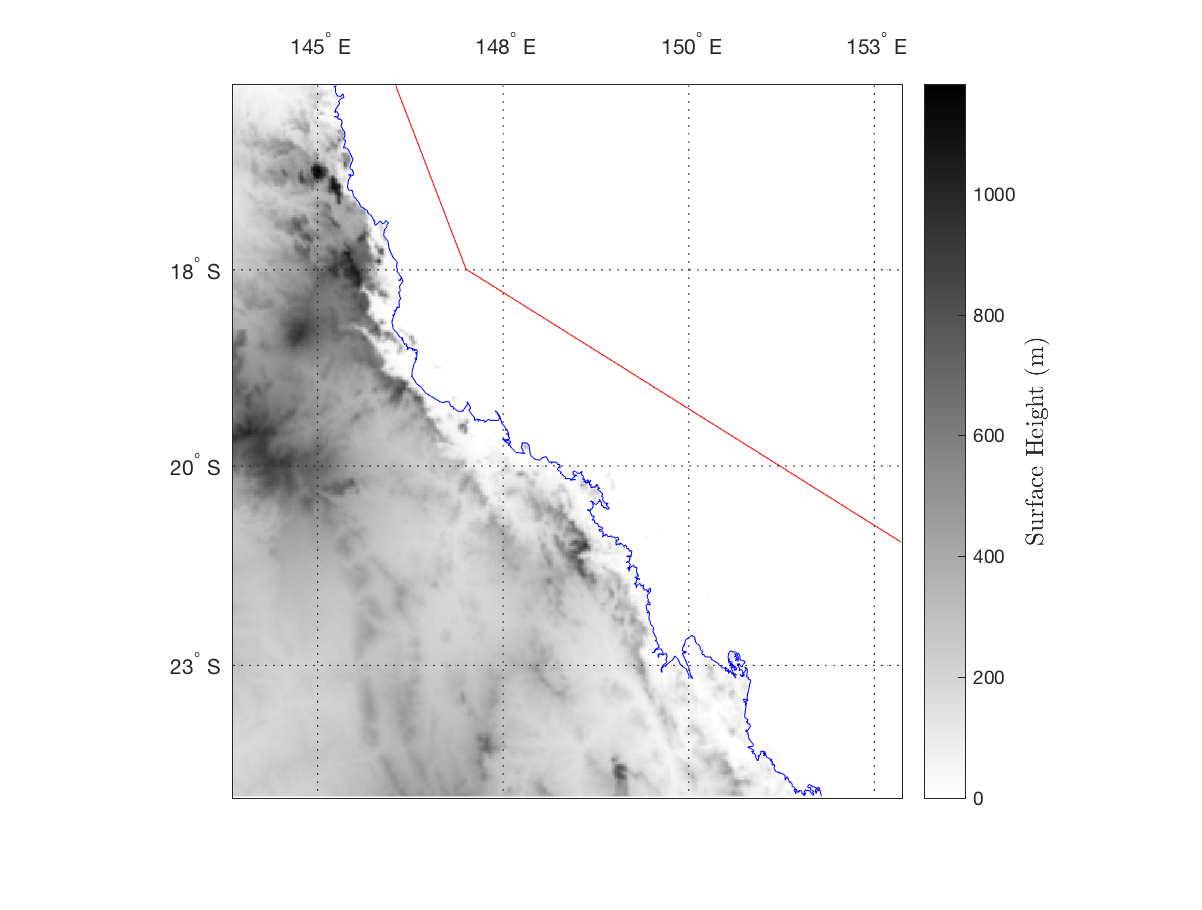
\includegraphics[width=0.8\textwidth]{Fig/Research/CCAM/TimeAveragedMap_zs.eps}
    \vspace{-1cm}
    \caption{ A map of the Height of the surface of the earth and ocean within the final \gls{ccam} domain. }
    \label{fig:zsmap}
\end{figure}

%------------------------------------------------------------------------------------------------------------------
\subsection{Air and Surface Temperatures}
\label{subsec:tempresults}

There are a number of different levels that temperatures can be sampled from. The five outputted pressure levels, the bottom pressure level the model simulated, the screen level (\SI{1.5}{\m} above the surface), and the surface temperature. These figures provide an image of what is happening with the air temperature within the simulated domain, over time, and how it varies vertically. The air temperature map in \cref{fig:tbotmap} contextualises the temperatures used in \cref{subsec:compplots}. The temperature over time for the \gls{gbr} in \cref{fig:tbottime} points to weather phenomena occurring during this month.

\begin{figure}[!hbt]
    \centering
    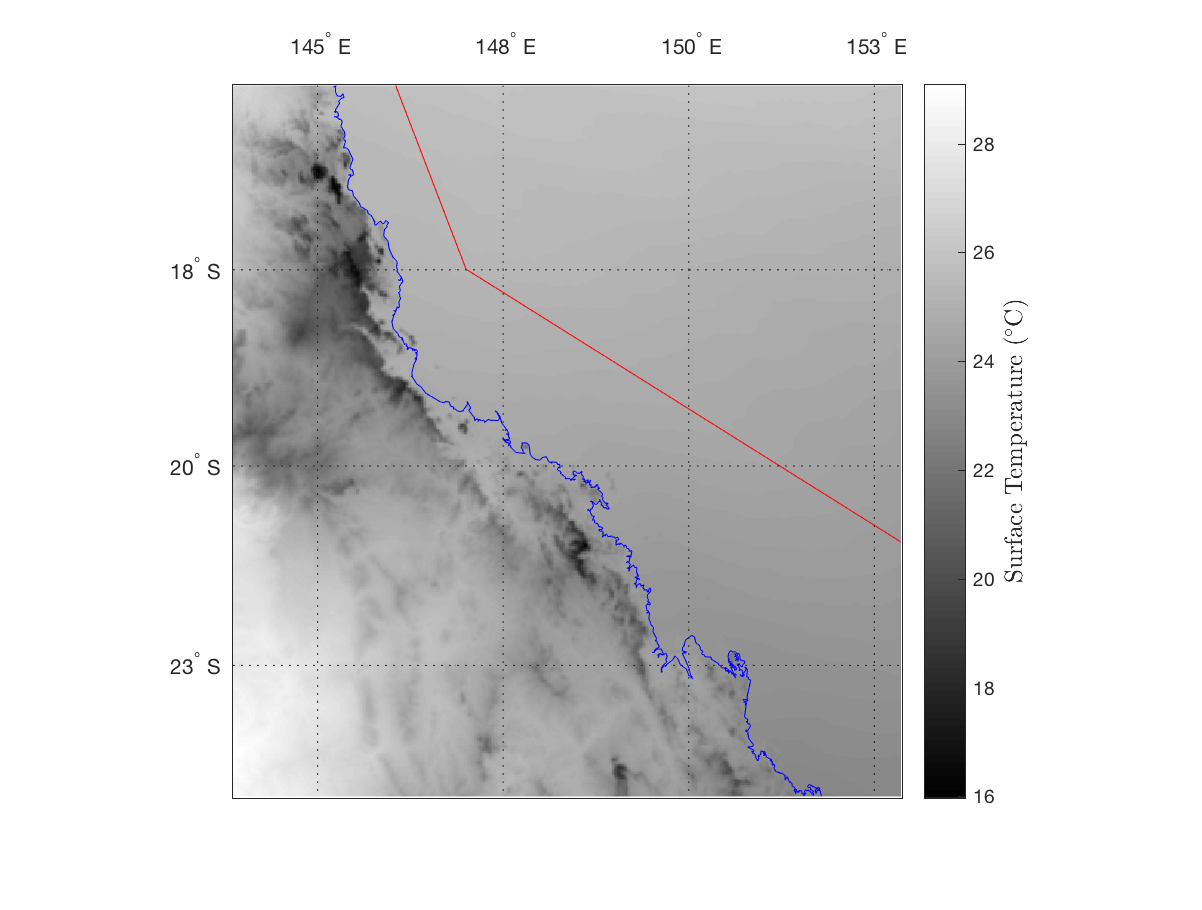
\includegraphics[width=0.8\textwidth]{Fig/Research/CCAM/TimeAveragedMap_tbot.eps}
    \vspace{-1cm}
    \caption{ A map of the Air Temperature at the lowest simulated Pressure level. The Temperatures were averaged over the modelled month, October 2015. }
    \label{fig:tbotmap}
\end{figure}

\begin{figure}[!hbt]
    \centering
    \includegraphics[width=0.7\textwidth]{Fig/Research/CCAM/GBRnTimeAveragedPlot_temp.eps}
    \caption{ The Air Temperature averaged from all points within the \gls{gbr} and also averaged over time then plotted against the modelled Pressure Levels. }
    \label{fig:tempvpress}
\end{figure}
\clearpage

\begin{figure}[!t]
    \centering
    \includegraphics[width=0.7\textwidth]{Fig/Research/CCAM/GBRAveragedPlot_tbot.eps}
    \caption{ The Air Temperature at the lowest simulated Pressure level, averaged from the points inside the \gls{gbr} region of the final \gls{ccam} domain. }
    \label{fig:tbottime}
\end{figure}


%------------------------------------------------------------------------------------------------------------------
\subsection{Wind Directions and Speed}
\label{subsec:windresults}

The wind in this system causes two of the main effects being examined. The first is the speed of the wind across the surface of the ocean as this is the largest influencing factor of \gls{dms} surface flux (see \cref{sec:dmssurf}). The second is in which direction and how far the \gls{dms} and its products are moved. These two points are illustrated in \cref{fig:magwind} and \cref{fig:windmap} respectively.

\begin{figure}[!hbt]
    \centering
    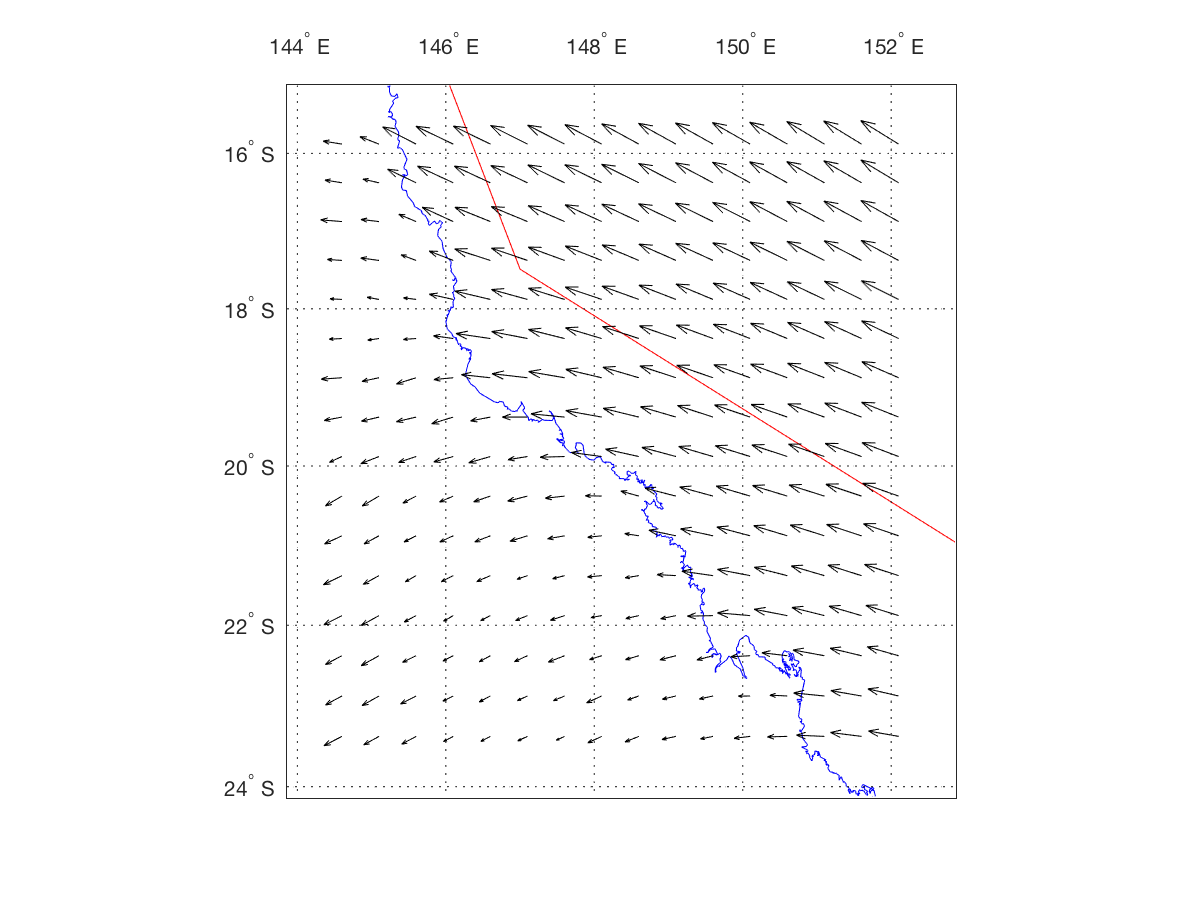
\includegraphics[width=0.75\textwidth]{Fig/Research/CCAM/WindSpeedMapAvgOverTime.eps}
    \vspace{-1cm}
    \caption{ A map of the final \gls{ccam} domain showing the modelled 10 metre Wind vectors. }
    \label{fig:windmap}
\end{figure}

\begin{figure}[!hbt]
    \centering
    \includegraphics[width=0.70\textwidth]{Fig/Research/CCAM/GBRAveragedPlot_u10.eps}
    \caption{ The magnitude of the 10 metre Wind Speed, averaged from the points inside the \gls{gbr} region of the final \gls{ccam} domain. }
    \label{fig:magwind}
\end{figure}

%------------------------------------------------------------------------------------------------------------------
\subsection{Clouds, Rain and Radiation}
\label{subsec:cloudsresults}

\gls{ccam} simulates three levels of cloud coverage as low, mid, and high cloud fraction. Combining these gives the total cloud fraction. The cloud coverage effects the amount of radiation hitting the surface of the earth. The radiation flux at the surface of the earth is composed of a number of source, direct, diffuse, reflected, and produced. Cloud coverage alters the fraction of direct and diffuse radiation. The net radiation at the surface of the \gls{gbr} can be see in \cref{fig:rnettime}. The cloud coverage also effects the presence of rain. In \cref{fig:rainmap} and in \cref{fig:cldmap} the rain fraction and total cloud fraction can be seen mapped to the modelled domain. This shows their distribution across the \gls{gbr}, but also along the Queensland coast.

\begin{figure}[!hbt]
    \centering
    \includegraphics[width=0.70\textwidth]{Fig/Research/CCAM/GBRAveragedPlot_cld.eps}
    \caption{ The Total Cloud Fraction, averaged from the points inside the \gls{gbr} region of the final \gls{ccam} domain. }
    \label{fig:cldtime}
\end{figure}

\begin{figure}[!hbt]
    \centering
    \includegraphics[width=0.70\textwidth]{Fig/Research/CCAM/GBRAveragedPlot_rnet_ave.eps}
    \caption{ The Net Radiation striking the surface, averaged from the points inside the \gls{gbr} region of the final \gls{ccam} domain. }
    \label{fig:rnettime}
\end{figure}

\begin{figure}[!hbt]
    \centering
    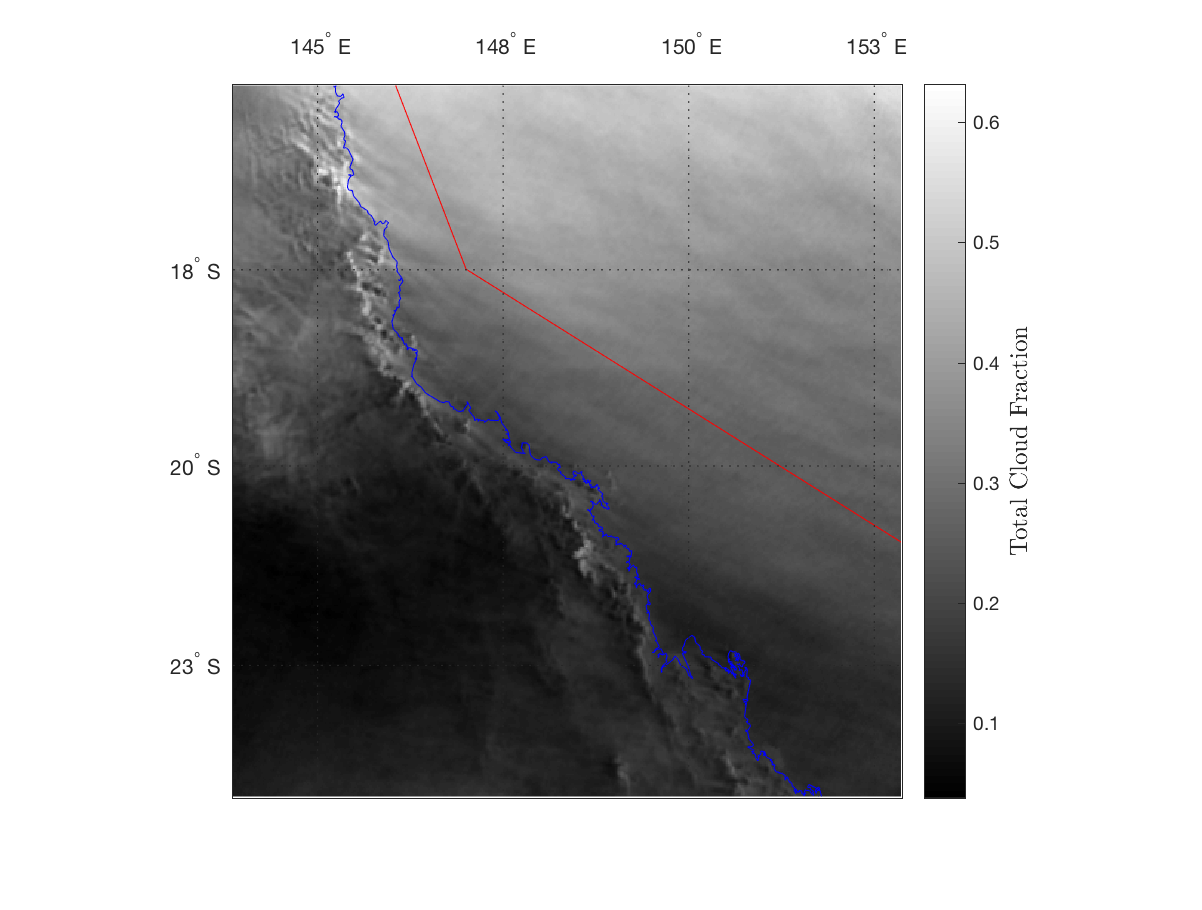
\includegraphics[width=0.8\textwidth]{Fig/Research/CCAM/TimeAveragedMap_cld.eps}
    \vspace{-1cm}
    \caption{ A map of the Total Cloud Fraction consisting of the Cloud Fractions from all levels. The Total Cloud fractions were averaged over the modelled month, October 2015. }
    \label{fig:cldmap}
\end{figure}

\begin{figure}[!hbt]
    \centering
    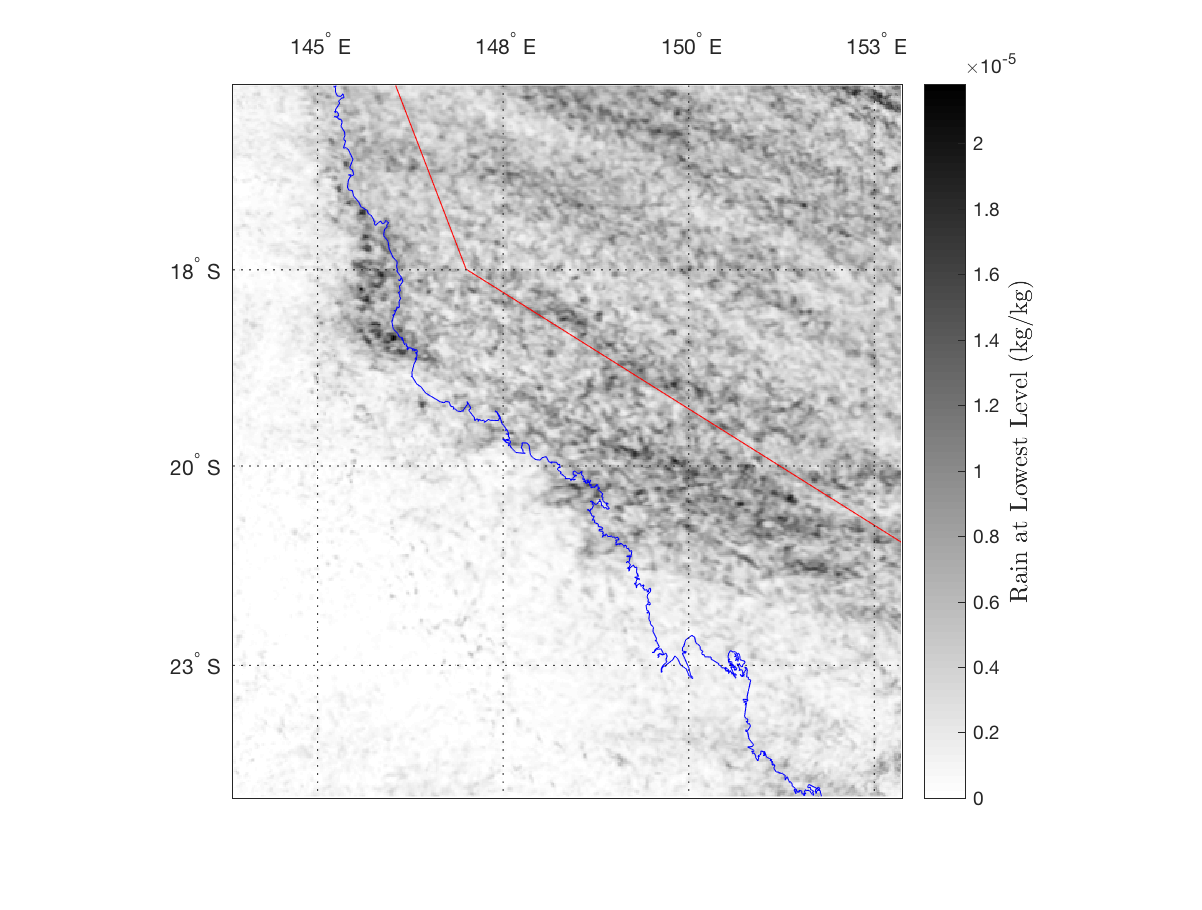
\includegraphics[width=0.8\textwidth]{Fig/Research/CCAM/TimeAveragedMap_qrg.eps}
    \vspace{-1cm}
    \caption{ A map of the Rain fraction at the 1000 hPa level of the model. The Rain fractions were averaged over the modelled month, October 2015. }
    \label{fig:rainmap}
\end{figure}

%------------------------------------------------------------------------------------------------------------------
% pressure	

